\documentclass[1p]{elsarticle_modified}
%\bibliographystyle{elsarticle-num}

%\usepackage[colorlinks]{hyperref}
%\usepackage{abbrmath_seonhwa} %\Abb, \Ascr, \Acal ,\Abf, \Afrak
\usepackage{amsfonts}
\usepackage{amssymb}
\usepackage{amsmath}
\usepackage{amsthm}
\usepackage{scalefnt}
\usepackage{amsbsy}
\usepackage{kotex}
\usepackage{caption}
\usepackage{subfig}
\usepackage{color}
\usepackage{graphicx}
\usepackage{xcolor} %% white, black, red, green, blue, cyan, magenta, yellow
\usepackage{float}
\usepackage{setspace}
\usepackage{hyperref}

\usepackage{tikz}
\usetikzlibrary{arrows}

\usepackage{multirow}
\usepackage{array} % fixed length table
\usepackage{hhline}

%%%%%%%%%%%%%%%%%%%%%
\makeatletter
\renewcommand*\env@matrix[1][\arraystretch]{%
	\edef\arraystretch{#1}%
	\hskip -\arraycolsep
	\let\@ifnextchar\new@ifnextchar
	\array{*\c@MaxMatrixCols c}}
\makeatother %https://tex.stackexchange.com/questions/14071/how-can-i-increase-the-line-spacing-in-a-matrix
%%%%%%%%%%%%%%%

\usepackage[normalem]{ulem}

\newcommand{\msout}[1]{\ifmmode\text{\sout{\ensuremath{#1}}}\else\sout{#1}\fi}
%SOURCE: \msout is \stkout macro in https://tex.stackexchange.com/questions/20609/strikeout-in-math-mode

\newcommand{\cancel}[1]{
	\ifmmode
	{\color{red}\msout{#1}}
	\else
	{\color{red}\sout{#1}}
	\fi
}

\newcommand{\add}[1]{
	{\color{blue}\uwave{#1}}
}

\newcommand{\replace}[2]{
	\ifmmode
	{\color{red}\msout{#1}}{\color{blue}\uwave{#2}}
	\else
	{\color{red}\sout{#1}}{\color{blue}\uwave{#2}}
	\fi
}

\newcommand{\Sol}{\mathcal{S}} %segment
\newcommand{\D}{D} %diagram
\newcommand{\A}{\mathcal{A}} %arc


%%%%%%%%%%%%%%%%%%%%%%%%%%%%%5 test

\def\sl{\operatorname{\textup{SL}}(2,\Cbb)}
\def\psl{\operatorname{\textup{PSL}}(2,\Cbb)}
\def\quan{\mkern 1mu \triangleright \mkern 1mu}

\theoremstyle{definition}
\newtheorem{thm}{Theorem}[section]
\newtheorem{prop}[thm]{Proposition}
\newtheorem{lem}[thm]{Lemma}
\newtheorem{ques}[thm]{Question}
\newtheorem{cor}[thm]{Corollary}
\newtheorem{defn}[thm]{Definition}
\newtheorem{exam}[thm]{Example}
\newtheorem{rmk}[thm]{Remark}
\newtheorem{alg}[thm]{Algorithm}

\newcommand{\I}{\sqrt{-1}}
\begin{document}

%\begin{frontmatter}
%
%\title{Boundary parabolic representations of knots up to 8 crossings}
%
%%% Group authors per affiliation:
%\author{Yunhi Cho} 
%\address{Department of Mathematics, University of Seoul, Seoul, Korea}
%\ead{yhcho@uos.ac.kr}
%
%
%\author{Seonhwa Kim} %\fnref{s_kim}}
%\address{Center for Geometry and Physics, Institute for Basic Science, Pohang, 37673, Korea}
%\ead{ryeona17@ibs.re.kr}
%
%\author{Hyuk Kim}
%\address{Department of Mathematical Sciences, Seoul National University, Seoul 08826, Korea}
%\ead{hyukkim@snu.ac.kr}
%
%\author{Seokbeom Yoon}
%\address{Department of Mathematical Sciences, Seoul National University, Seoul, 08826,  Korea}
%\ead{sbyoon15@snu.ac.kr}
%
%\begin{abstract}
%We find all boundary parabolic representation of knots up to 8 crossings.
%
%\end{abstract}
%\begin{keyword}
%    \MSC[2010] 57M25 
%\end{keyword}
%
%\end{frontmatter}

%\linenumbers
%\tableofcontents
%
\newcommand\colored[1]{\textcolor{white}{\rule[-0.35ex]{0.8em}{1.4ex}}\kern-0.8em\color{red} #1}%
%\newcommand\colored[1]{\textcolor{white}{ #1}\kern-2.17ex	\textcolor{white}{ #1}\kern-1.81ex	\textcolor{white}{ #1}\kern-2.15ex\color{red}#1	}

{\Large $\underline{12a_{0907}~(K12a_{0907})}$}

\setlength{\tabcolsep}{10pt}
\renewcommand{\arraystretch}{1.6}
\vspace{1cm}\begin{tabular}{m{100pt}>{\centering\arraybackslash}m{274pt}}
\multirow{5}{120pt}{
	\centering
	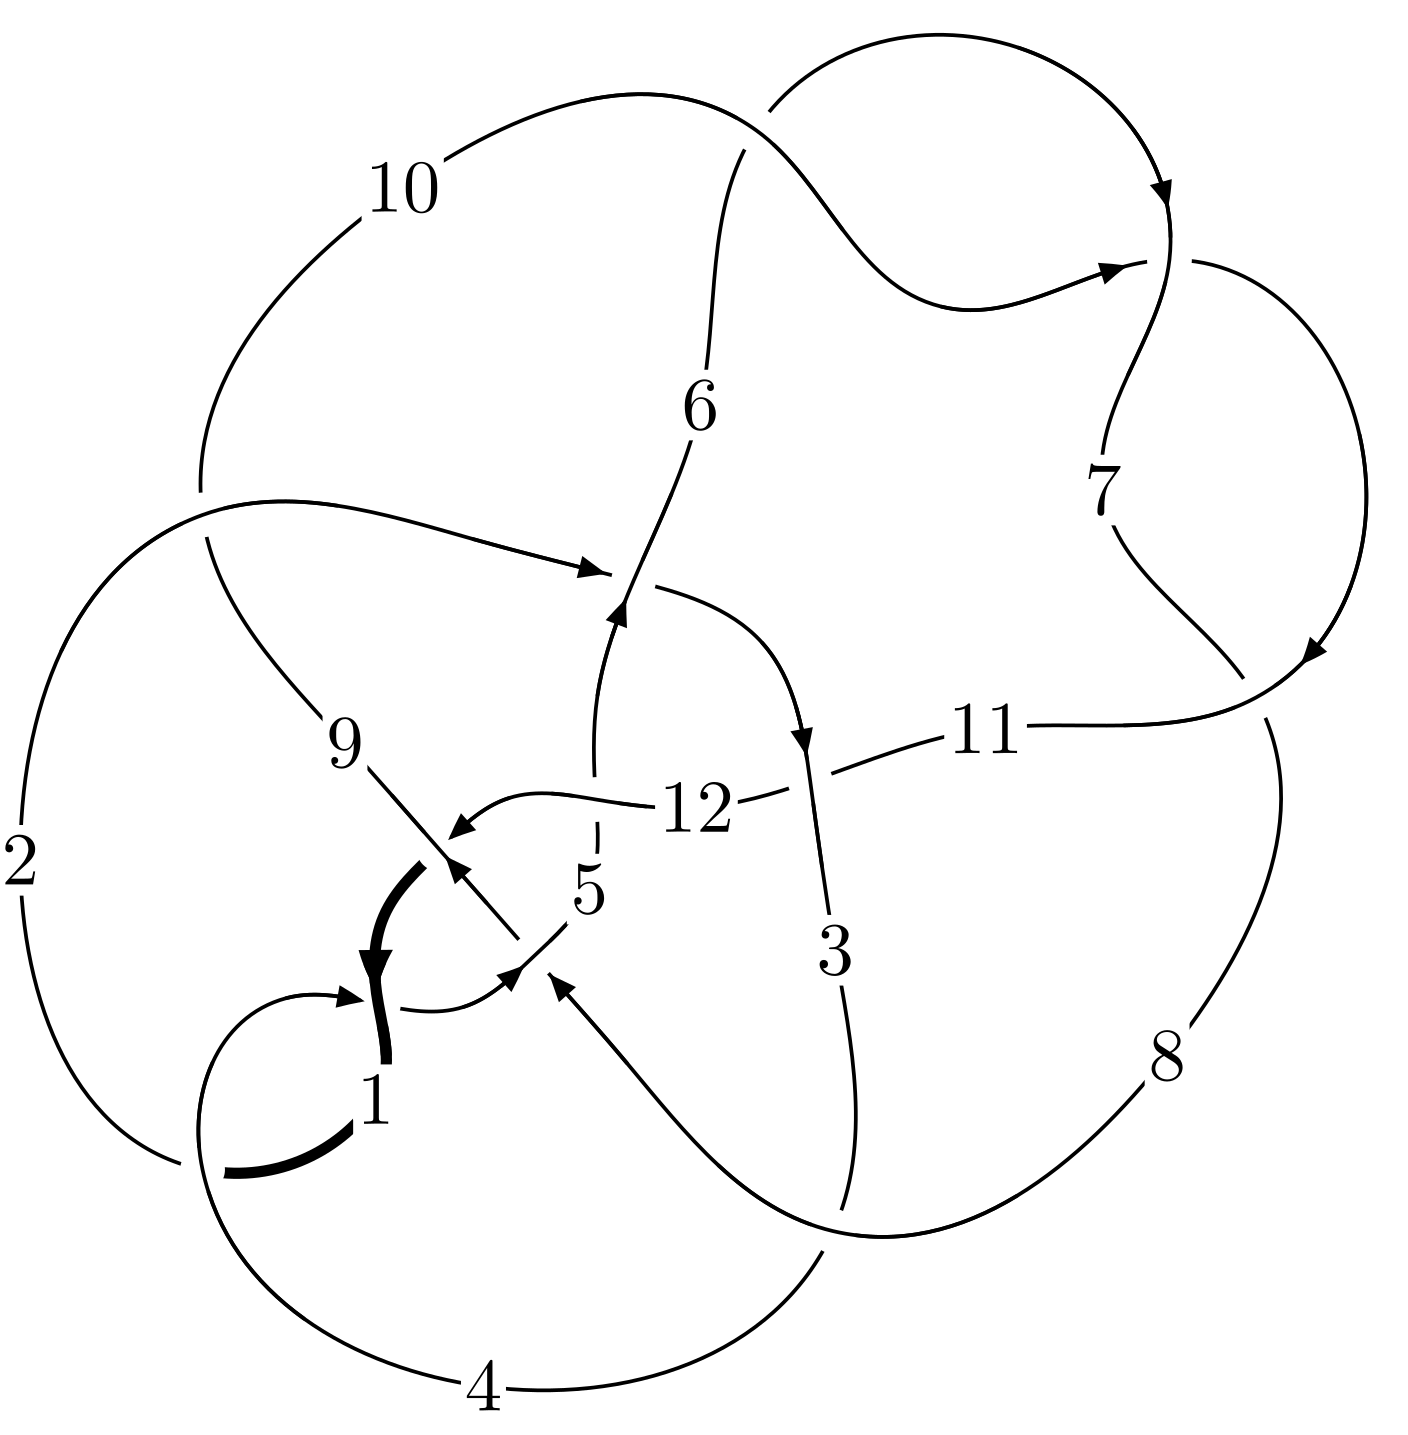
\includegraphics[width=112pt]{../../../GIT/diagram.site/Diagrams/png/1708_12a_0907.png}\\
\ \ \ A knot diagram\footnotemark}&
\allowdisplaybreaks
\textbf{Linearized knot diagam} \\
\cline{2-2}
 &
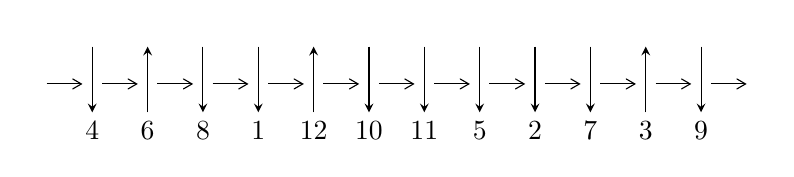
\begin{tikzpicture}[x=20pt, y=17pt]
	% nodes
	\node (C0) at (0, 0) {};
	\node (C1) at (1, 0) {};
	\node (C1U) at (1, +1) {};
	\node (C1D) at (1, -1) {4};

	\node (C2) at (2, 0) {};
	\node (C2U) at (2, +1) {};
	\node (C2D) at (2, -1) {6};

	\node (C3) at (3, 0) {};
	\node (C3U) at (3, +1) {};
	\node (C3D) at (3, -1) {8};

	\node (C4) at (4, 0) {};
	\node (C4U) at (4, +1) {};
	\node (C4D) at (4, -1) {1};

	\node (C5) at (5, 0) {};
	\node (C5U) at (5, +1) {};
	\node (C5D) at (5, -1) {12};

	\node (C6) at (6, 0) {};
	\node (C6U) at (6, +1) {};
	\node (C6D) at (6, -1) {10};

	\node (C7) at (7, 0) {};
	\node (C7U) at (7, +1) {};
	\node (C7D) at (7, -1) {11};

	\node (C8) at (8, 0) {};
	\node (C8U) at (8, +1) {};
	\node (C8D) at (8, -1) {5};

	\node (C9) at (9, 0) {};
	\node (C9U) at (9, +1) {};
	\node (C9D) at (9, -1) {2};

	\node (C10) at (10, 0) {};
	\node (C10U) at (10, +1) {};
	\node (C10D) at (10, -1) {7};

	\node (C11) at (11, 0) {};
	\node (C11U) at (11, +1) {};
	\node (C11D) at (11, -1) {3};

	\node (C12) at (12, 0) {};
	\node (C12U) at (12, +1) {};
	\node (C12D) at (12, -1) {9};
	\node (C13) at (13, 0) {};

	% arrows
	\draw[->,>={angle 60}]
	(C0) edge (C1) (C1) edge (C2) (C2) edge (C3) (C3) edge (C4) (C4) edge (C5) (C5) edge (C6) (C6) edge (C7) (C7) edge (C8) (C8) edge (C9) (C9) edge (C10) (C10) edge (C11) (C11) edge (C12) (C12) edge (C13) ;	\draw[->,>=stealth]
	(C1U) edge (C1D) (C2D) edge (C2U) (C3U) edge (C3D) (C4U) edge (C4D) (C5D) edge (C5U) (C6U) edge (C6D) (C7U) edge (C7D) (C8U) edge (C8D) (C9U) edge (C9D) (C10U) edge (C10D) (C11D) edge (C11U) (C12U) edge (C12D) ;
	\end{tikzpicture} \\
\hhline{~~} \\& 
\textbf{Solving Sequence} \\ \cline{2-2} 
 &
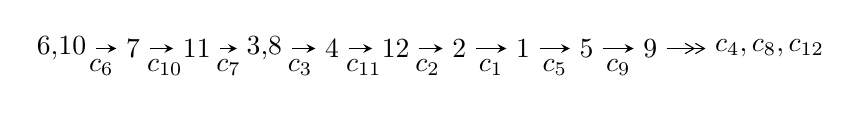
\begin{tikzpicture}[x=23pt, y=7pt]
	% node
	\node (A0) at (-1/8, 0) {6,10};
	\node (A1) at (1, 0) {7};
	\node (A2) at (2, 0) {11};
	\node (A3) at (49/16, 0) {3,8};
	\node (A4) at (33/8, 0) {4};
	\node (A5) at (41/8, 0) {12};
	\node (A6) at (49/8, 0) {2};
	\node (A7) at (57/8, 0) {1};
	\node (A8) at (65/8, 0) {5};
	\node (A9) at (73/8, 0) {9};
	\node (C1) at (1/2, -1) {$c_{6}$};
	\node (C2) at (3/2, -1) {$c_{10}$};
	\node (C3) at (5/2, -1) {$c_{7}$};
	\node (C4) at (29/8, -1) {$c_{3}$};
	\node (C5) at (37/8, -1) {$c_{11}$};
	\node (C6) at (45/8, -1) {$c_{2}$};
	\node (C7) at (53/8, -1) {$c_{1}$};
	\node (C8) at (61/8, -1) {$c_{5}$};
	\node (C9) at (69/8, -1) {$c_{9}$};
	\node (A10) at (11, 0) {$c_{4},c_{8},c_{12}$};

	% edge
	\draw[->,>=stealth]	
	(A0) edge (A1) (A1) edge (A2) (A2) edge (A3) (A3) edge (A4) (A4) edge (A5) (A5) edge (A6) (A6) edge (A7) (A7) edge (A8) (A8) edge (A9) ;
	\draw[->>,>={angle 60}]	
	(A9) edge (A10);
\end{tikzpicture} \\ 

\end{tabular} \\

\footnotetext{
The image of knot diagram is generated by the software ``\textbf{Draw programme}" developed by Andrew Bartholomew(\url{http://www.layer8.co.uk/maths/draw/index.htm\#Running-draw}), where we modified some parts for our purpose(\url{https://github.com/CATsTAILs/LinksPainter}).
}\phantom \\ \newline 
\centering \textbf{Ideals for irreducible components\footnotemark of $X_{\text{par}}$} 
 
\begin{align*}
I^u_{1}&=\langle 
-3.36776\times10^{26} u^{53}+3.91730\times10^{27} u^{52}+\cdots+2.24514\times10^{23} b-9.81393\times10^{26},\\
\phantom{I^u_{1}}&\phantom{= \langle  }-1.27427\times10^{27} u^{53}+1.48006\times10^{28} u^{52}+\cdots+4.49027\times10^{23} a-3.66919\times10^{27},\\
\phantom{I^u_{1}}&\phantom{= \langle  }u^{54}-13 u^{53}+\cdots+34 u-4\rangle \\
I^u_{2}&=\langle 
686725223456 u^{23} a^3-53855889828079 u^{23} a^2+\cdots-122527711835341 a-257682162174646,\\
\phantom{I^u_{2}}&\phantom{= \langle  }7 u^{23} a^3-30 u^{23} a^2+\cdots+101 a+65,\;u^{24}+3 u^{23}+\cdots-3 u-1\rangle \\
I^u_{3}&=\langle 
-1133664 u^{29}-7205220 u^{28}+\cdots+38189 b-689951,\\
\phantom{I^u_{3}}&\phantom{= \langle  }-233434 u^{29}-944087 u^{28}+\cdots+38189 a+273567,\;u^{30}+8 u^{29}+\cdots+6 u+1\rangle \\
I^u_{4}&=\langle 
-2 a^7+19 a^6+18 a^5-57 a^4-111 a^3+159 a^2+55 b+6 a-61,\\
\phantom{I^u_{4}}&\phantom{= \langle  }a^8-3 a^6-2 a^5+10 a^4-6 a^3-2 a^2+2 a+1,\;u-1\rangle \\
\\
\end{align*}
\raggedright * 4 irreducible components of $\dim_{\mathbb{C}}=0$, with total 188 representations.\\
\footnotetext{All coefficients of polynomials are rational numbers. But the coefficients are sometimes approximated in decimal forms when there is not enough margin.}
\newpage
\renewcommand{\arraystretch}{1}
\centering \section*{I. $I^u_{1}= \langle -3.37\times10^{26} u^{53}+3.92\times10^{27} u^{52}+\cdots+2.25\times10^{23} b-9.81\times10^{26},\;-1.27\times10^{27} u^{53}+1.48\times10^{28} u^{52}+\cdots+4.49\times10^{23} a-3.67\times10^{27},\;u^{54}-13 u^{53}+\cdots+34 u-4 \rangle$}
\flushleft \textbf{(i) Arc colorings}\\
\begin{tabular}{m{7pt} m{180pt} m{7pt} m{180pt} }
\flushright $a_{6}=$&$\begin{pmatrix}1\\0\end{pmatrix}$ \\
\flushright $a_{10}=$&$\begin{pmatrix}0\\u\end{pmatrix}$ \\
\flushright $a_{7}=$&$\begin{pmatrix}1\\u^2\end{pmatrix}$ \\
\flushright $a_{11}=$&$\begin{pmatrix}- u\\- u^3+u\end{pmatrix}$ \\
\flushright $a_{3}=$&$\begin{pmatrix}2837.85 u^{53}-32961.4 u^{52}+\cdots-63640.3 u+8171.42\\1500.03 u^{53}-17447.9 u^{52}+\cdots-33975.2 u+4371.20\end{pmatrix}$ \\
\flushright $a_{8}=$&$\begin{pmatrix}- u^2+1\\- u^4+2 u^2\end{pmatrix}$ \\
\flushright $a_{4}=$&$\begin{pmatrix}1040.34 u^{53}-12078.0 u^{52}+\cdots-23374.2 u+2997.45\\1765.41 u^{53}-20426.7 u^{52}+\cdots-38653.6 u+4959.58\end{pmatrix}$ \\
\flushright $a_{12}=$&$\begin{pmatrix}700.056 u^{53}-8023.67 u^{52}+\cdots-14095.8 u+1795.50\\561.272 u^{53}-6465.23 u^{52}+\cdots-11812.3 u+1508.00\end{pmatrix}$ \\
\flushright $a_{2}=$&$\begin{pmatrix}1337.82 u^{53}-15513.4 u^{52}+\cdots-29665.1 u+3800.22\\1500.03 u^{53}-17447.9 u^{52}+\cdots-33975.2 u+4371.20\end{pmatrix}$ \\
\flushright $a_{1}=$&$\begin{pmatrix}1322.69 u^{53}-15354.9 u^{52}+\cdots-29533.0 u+3779.67\\1634.57 u^{53}-18951.8 u^{52}+\cdots-36197.1 u+4648.23\end{pmatrix}$ \\
\flushright $a_{5}=$&$\begin{pmatrix}-1168.57 u^{53}+13437.1 u^{52}+\cdots+24303.1 u-3094.58\\-1266.34 u^{53}+14590.7 u^{52}+\cdots+26781.1 u-3423.17\end{pmatrix}$ \\
\flushright $a_{9}=$&$\begin{pmatrix}264.065 u^{53}-3140.74 u^{52}+\cdots-6974.68 u+915.893\\-245.749 u^{53}+2782.17 u^{52}+\cdots+4432.15 u-555.135\end{pmatrix}$\\&\end{tabular}
\flushleft \textbf{(ii) Obstruction class $= -1$}\\~\\
\flushleft \textbf{(iii) Cusp Shapes $= \frac{589994116974512942783147236}{112256792457085332631919} u^{53}-\frac{6776033072646746153986440530}{112256792457085332631919} u^{52}+\cdots-\frac{12142947172972580665078190700}{112256792457085332631919} u+\frac{1547202967534202217337683890}{112256792457085332631919}$}\\~\\
\newpage\renewcommand{\arraystretch}{1}
\flushleft \textbf{(iv) u-Polynomials at the component}\newline \\
\begin{tabular}{m{50pt}|m{274pt}}
Crossings & \hspace{64pt}u-Polynomials at each crossing \\
\hline $$\begin{aligned}c_{1},c_{4}\end{aligned}$$&$\begin{aligned}
&u^{54}-22 u^{53}+\cdots-4312 u+448
\end{aligned}$\\
\hline $$\begin{aligned}c_{2},c_{11}\end{aligned}$$&$\begin{aligned}
&u^{54}- u^{53}+\cdots+13 u+2
\end{aligned}$\\
\hline $$\begin{aligned}c_{3},c_{9}\end{aligned}$$&$\begin{aligned}
&u^{54}- u^{53}+\cdots+28 u-4
\end{aligned}$\\
\hline $$\begin{aligned}c_{5}\end{aligned}$$&$\begin{aligned}
&u^{54}-45 u^{53}+\cdots-144703488 u+8388608
\end{aligned}$\\
\hline $$\begin{aligned}c_{6},c_{7},c_{10}\end{aligned}$$&$\begin{aligned}
&u^{54}+13 u^{53}+\cdots-34 u-4
\end{aligned}$\\
\hline $$\begin{aligned}c_{8},c_{12}\end{aligned}$$&$\begin{aligned}
&u^{54}+u^{53}+\cdots- u-1
\end{aligned}$\\
\hline
\end{tabular}\\~\\
\newpage\renewcommand{\arraystretch}{1}
\flushleft \textbf{(v) Riley Polynomials at the component}\newline \\
\begin{tabular}{m{50pt}|m{274pt}}
Crossings & \hspace{64pt}Riley Polynomials at each crossing \\
\hline $$\begin{aligned}c_{1},c_{4}\end{aligned}$$&$\begin{aligned}
&y^{54}+36 y^{53}+\cdots+1750336 y+200704
\end{aligned}$\\
\hline $$\begin{aligned}c_{2},c_{11}\end{aligned}$$&$\begin{aligned}
&y^{54}+9 y^{53}+\cdots+83 y+4
\end{aligned}$\\
\hline $$\begin{aligned}c_{3},c_{9}\end{aligned}$$&$\begin{aligned}
&y^{54}-27 y^{53}+\cdots-896 y+16
\end{aligned}$\\
\hline $$\begin{aligned}c_{5}\end{aligned}$$&$\begin{aligned}
&y^{54}+5 y^{53}+\cdots-532163627843584 y+70368744177664
\end{aligned}$\\
\hline $$\begin{aligned}c_{6},c_{7},c_{10}\end{aligned}$$&$\begin{aligned}
&y^{54}-55 y^{53}+\cdots-908 y+16
\end{aligned}$\\
\hline $$\begin{aligned}c_{8},c_{12}\end{aligned}$$&$\begin{aligned}
&y^{54}+23 y^{53}+\cdots+31 y+1
\end{aligned}$\\
\hline
\end{tabular}\\~\\
\newpage\flushleft \textbf{(vi) Complex Volumes and Cusp Shapes}
$$\begin{array}{c|c|c}  
\text{Solutions to }I^u_{1}& \I (\text{vol} + \sqrt{-1}CS) & \text{Cusp shape}\\
 \hline 
\begin{aligned}
u &= -0.441312 + 0.889865 I \\
a &= \phantom{-}0.480858 + 0.262881 I \\
b &= \phantom{-}0.365486 - 0.846526 I\end{aligned}
 & -3.91979 - 4.10130 I & \phantom{-0.000000 } 0 \\ \hline\begin{aligned}
u &= -0.441312 - 0.889865 I \\
a &= \phantom{-}0.480858 - 0.262881 I \\
b &= \phantom{-}0.365486 + 0.846526 I\end{aligned}
 & -3.91979 + 4.10130 I & \phantom{-0.000000 } 0 \\ \hline\begin{aligned}
u &= -0.570988 + 0.834174 I \\
a &= \phantom{-}0.608929 - 0.543849 I \\
b &= -0.84924 - 1.19743 I\end{aligned}
 & -1.0568 + 15.5175 I & \phantom{-0.000000 } 0 \\ \hline\begin{aligned}
u &= -0.570988 - 0.834174 I \\
a &= \phantom{-}0.608929 + 0.543849 I \\
b &= -0.84924 + 1.19743 I\end{aligned}
 & -1.0568 - 15.5175 I & \phantom{-0.000000 } 0 \\ \hline\begin{aligned}
u &= -0.637135 + 0.741301 I \\
a &= -0.476946 + 0.620063 I \\
b &= \phantom{-}0.809980 + 1.110120 I\end{aligned}
 & -4.60432 + 9.42368 I & \phantom{-0.000000 } 0 \\ \hline\begin{aligned}
u &= -0.637135 - 0.741301 I \\
a &= -0.476946 - 0.620063 I \\
b &= \phantom{-}0.809980 - 1.110120 I\end{aligned}
 & -4.60432 - 9.42368 I & \phantom{-0.000000 } 0 \\ \hline\begin{aligned}
u &= -0.608693 + 0.871804 I \\
a &= -0.547448 - 0.169996 I \\
b &= -0.448601 + 1.021030 I\end{aligned}
 & -1.09490 - 9.86752 I & \phantom{-0.000000 } 0 \\ \hline\begin{aligned}
u &= -0.608693 - 0.871804 I \\
a &= -0.547448 + 0.169996 I \\
b &= -0.448601 - 1.021030 I\end{aligned}
 & -1.09490 + 9.86752 I & \phantom{-0.000000 } 0 \\ \hline\begin{aligned}
u &= \phantom{-}0.900779 + 0.233525 I \\
a &= -0.574933 + 0.544624 I \\
b &= -0.019206 - 0.185995 I\end{aligned}
 & -0.294416 - 0.269624 I & \phantom{-0.000000 } 0 \\ \hline\begin{aligned}
u &= \phantom{-}0.900779 - 0.233525 I \\
a &= -0.574933 - 0.544624 I \\
b &= -0.019206 + 0.185995 I\end{aligned}
 & -0.294416 + 0.269624 I & \phantom{-0.000000 } 0\\
 \hline 
 \end{array}$$\newpage$$\begin{array}{c|c|c}  
\text{Solutions to }I^u_{1}& \I (\text{vol} + \sqrt{-1}CS) & \text{Cusp shape}\\
 \hline 
\begin{aligned}
u &= -0.990203 + 0.557417 I \\
a &= \phantom{-}0.284165 + 0.146019 I \\
b &= \phantom{-}0.714298 - 0.229702 I\end{aligned}
 & \phantom{-}3.53531 + 5.84821 I & \phantom{-0.000000 } 0 \\ \hline\begin{aligned}
u &= -0.990203 - 0.557417 I \\
a &= \phantom{-}0.284165 - 0.146019 I \\
b &= \phantom{-}0.714298 + 0.229702 I\end{aligned}
 & \phantom{-}3.53531 - 5.84821 I & \phantom{-0.000000 } 0 \\ \hline\begin{aligned}
u &= -0.637541 + 0.994808 I \\
a &= -0.267203 + 0.183692 I \\
b &= \phantom{-}0.401222 + 0.614737 I\end{aligned}
 & \phantom{-}2.70452 + 6.50099 I & \phantom{-0.000000 } 0 \\ \hline\begin{aligned}
u &= -0.637541 - 0.994808 I \\
a &= -0.267203 - 0.183692 I \\
b &= \phantom{-}0.401222 - 0.614737 I\end{aligned}
 & \phantom{-}2.70452 - 6.50099 I & \phantom{-0.000000 } 0 \\ \hline\begin{aligned}
u &= -0.232302 + 0.697717 I \\
a &= -0.546747 + 0.697335 I \\
b &= \phantom{-}0.822239 + 0.418863 I\end{aligned}
 & \phantom{-}5.64709 - 1.46866 I & \phantom{-0.000000 } 0 \\ \hline\begin{aligned}
u &= -0.232302 - 0.697717 I \\
a &= -0.546747 - 0.697335 I \\
b &= \phantom{-}0.822239 - 0.418863 I\end{aligned}
 & \phantom{-}5.64709 + 1.46866 I & \phantom{-0.000000 } 0 \\ \hline\begin{aligned}
u &= -0.910231 + 0.907970 I \\
a &= \phantom{-}0.175775 - 0.131869 I \\
b &= -0.176983 - 0.570715 I\end{aligned}
 & \phantom{-}1.99463 + 0.20661 I & \phantom{-0.000000 } 0 \\ \hline\begin{aligned}
u &= -0.910231 - 0.907970 I \\
a &= \phantom{-}0.175775 + 0.131869 I \\
b &= -0.176983 + 0.570715 I\end{aligned}
 & \phantom{-}1.99463 - 0.20661 I & \phantom{-0.000000 } 0 \\ \hline\begin{aligned}
u &= \phantom{-}1.339880 + 0.030929 I \\
a &= \phantom{-}1.23977 + 1.88630 I \\
b &= \phantom{-}0.465396 + 0.921605 I\end{aligned}
 & -2.39574 + 1.99510 I & \phantom{-0.000000 } 0 \\ \hline\begin{aligned}
u &= \phantom{-}1.339880 - 0.030929 I \\
a &= \phantom{-}1.23977 - 1.88630 I \\
b &= \phantom{-}0.465396 - 0.921605 I\end{aligned}
 & -2.39574 - 1.99510 I & \phantom{-0.000000 } 0\\
 \hline 
 \end{array}$$\newpage$$\begin{array}{c|c|c}  
\text{Solutions to }I^u_{1}& \I (\text{vol} + \sqrt{-1}CS) & \text{Cusp shape}\\
 \hline 
\begin{aligned}
u &= -0.476300 + 0.421762 I \\
a &= \phantom{-}0.402419 - 1.333210 I \\
b &= -0.886558 - 1.031710 I\end{aligned}
 & \phantom{-}1.45632 + 3.89302 I & \phantom{-}6.55672 - 9.08244 I \\ \hline\begin{aligned}
u &= -0.476300 - 0.421762 I \\
a &= \phantom{-}0.402419 + 1.333210 I \\
b &= -0.886558 + 1.031710 I\end{aligned}
 & \phantom{-}1.45632 - 3.89302 I & \phantom{-}6.55672 + 9.08244 I \\ \hline\begin{aligned}
u &= \phantom{-}1.378770 + 0.190230 I \\
a &= \phantom{-}0.08077 - 1.62497 I \\
b &= \phantom{-}0.582543 - 0.762799 I\end{aligned}
 & \phantom{-}0.56954 - 1.63715 I & \phantom{-0.000000 } 0 \\ \hline\begin{aligned}
u &= \phantom{-}1.378770 - 0.190230 I \\
a &= \phantom{-}0.08077 + 1.62497 I \\
b &= \phantom{-}0.582543 + 0.762799 I\end{aligned}
 & \phantom{-}0.56954 + 1.63715 I & \phantom{-0.000000 } 0 \\ \hline\begin{aligned}
u &= -0.503257 + 0.340699 I \\
a &= -0.308311 - 0.871589 I \\
b &= -0.793291 - 0.347440 I\end{aligned}
 & \phantom{-}1.42449 + 1.40957 I & \phantom{-}1.24500 - 4.46886 I \\ \hline\begin{aligned}
u &= -0.503257 - 0.340699 I \\
a &= -0.308311 + 0.871589 I \\
b &= -0.793291 + 0.347440 I\end{aligned}
 & \phantom{-}1.42449 - 1.40957 I & \phantom{-}1.24500 + 4.46886 I \\ \hline\begin{aligned}
u &= -1.42698 + 0.05858 I \\
a &= -0.411356 - 0.061254 I \\
b &= -1.43704 - 0.11906 I\end{aligned}
 & -3.13163 + 3.14235 I & \phantom{-0.000000 } 0 \\ \hline\begin{aligned}
u &= -1.42698 - 0.05858 I \\
a &= -0.411356 + 0.061254 I \\
b &= -1.43704 + 0.11906 I\end{aligned}
 & -3.13163 - 3.14235 I & \phantom{-0.000000 } 0 \\ \hline\begin{aligned}
u &= \phantom{-}0.565586\phantom{ +0.000000I} \\
a &= -0.656550\phantom{ +0.000000I} \\
b &= \phantom{-}0.161313\phantom{ +0.000000I}\end{aligned}
 & -0.821914\phantom{ +0.000000I} & -12.3890\phantom{ +0.000000I} \\ \hline\begin{aligned}
u &= -1.44155 + 0.03373 I \\
a &= \phantom{-}0.431824 - 0.086075 I \\
b &= \phantom{-}1.50809 - 0.35940 I\end{aligned}
 & -3.83782 - 1.54660 I & \phantom{-0.000000 } 0\\
 \hline 
 \end{array}$$\newpage$$\begin{array}{c|c|c}  
\text{Solutions to }I^u_{1}& \I (\text{vol} + \sqrt{-1}CS) & \text{Cusp shape}\\
 \hline 
\begin{aligned}
u &= -1.44155 - 0.03373 I \\
a &= \phantom{-}0.431824 + 0.086075 I \\
b &= \phantom{-}1.50809 + 0.35940 I\end{aligned}
 & -3.83782 + 1.54660 I & \phantom{-0.000000 } 0 \\ \hline\begin{aligned}
u &= \phantom{-}1.44478 + 0.02804 I \\
a &= -0.49400 + 1.70003 I \\
b &= -0.407113 + 1.064940 I\end{aligned}
 & -4.61801 - 2.16208 I & \phantom{-0.000000 } 0 \\ \hline\begin{aligned}
u &= \phantom{-}1.44478 - 0.02804 I \\
a &= -0.49400 - 1.70003 I \\
b &= -0.407113 - 1.064940 I\end{aligned}
 & -4.61801 + 2.16208 I & \phantom{-0.000000 } 0 \\ \hline\begin{aligned}
u &= -0.502533 + 0.069201 I \\
a &= -1.248020 + 0.506640 I \\
b &= -0.866071 + 0.553290 I\end{aligned}
 & \phantom{-}1.43237 - 1.61761 I & \phantom{-}1.66182 + 0.91579 I \\ \hline\begin{aligned}
u &= -0.502533 - 0.069201 I \\
a &= -1.248020 - 0.506640 I \\
b &= -0.866071 - 0.553290 I\end{aligned}
 & \phantom{-}1.43237 + 1.61761 I & \phantom{-}1.66182 - 0.91579 I \\ \hline\begin{aligned}
u &= \phantom{-}1.52443 + 0.12641 I \\
a &= -0.41871 + 2.19083 I \\
b &= -0.89545 + 1.60801 I\end{aligned}
 & -5.24335 - 5.87061 I & \phantom{-0.000000 } 0 \\ \hline\begin{aligned}
u &= \phantom{-}1.52443 - 0.12641 I \\
a &= -0.41871 - 2.19083 I \\
b &= -0.89545 - 1.60801 I\end{aligned}
 & -5.24335 + 5.87061 I & \phantom{-0.000000 } 0 \\ \hline\begin{aligned}
u &= -1.56753\phantom{ +0.000000I} \\
a &= \phantom{-}0.225076\phantom{ +0.000000I} \\
b &= \phantom{-}0.905857\phantom{ +0.000000I}\end{aligned}
 & -8.29018\phantom{ +0.000000I} & \phantom{-0.000000 } 0 \\ \hline\begin{aligned}
u &= \phantom{-}1.55862 + 0.28807 I \\
a &= \phantom{-}0.04358 + 1.83178 I \\
b &= -1.08291 + 1.46947 I\end{aligned}
 & -8.0087 - 19.6385 I & \phantom{-0.000000 } 0 \\ \hline\begin{aligned}
u &= \phantom{-}1.55862 - 0.28807 I \\
a &= \phantom{-}0.04358 - 1.83178 I \\
b &= -1.08291 - 1.46947 I\end{aligned}
 & -8.0087 + 19.6385 I & \phantom{-0.000000 } 0\\
 \hline 
 \end{array}$$\newpage$$\begin{array}{c|c|c}  
\text{Solutions to }I^u_{1}& \I (\text{vol} + \sqrt{-1}CS) & \text{Cusp shape}\\
 \hline 
\begin{aligned}
u &= \phantom{-}1.57042 + 0.24408 I \\
a &= \phantom{-}0.09505 - 1.82694 I \\
b &= \phantom{-}1.03413 - 1.47804 I\end{aligned}
 & -11.8661 - 13.0652 I & \phantom{-0.000000 } 0 \\ \hline\begin{aligned}
u &= \phantom{-}1.57042 - 0.24408 I \\
a &= \phantom{-}0.09505 + 1.82694 I \\
b &= \phantom{-}1.03413 + 1.47804 I\end{aligned}
 & -11.8661 + 13.0652 I & \phantom{-0.000000 } 0 \\ \hline\begin{aligned}
u &= \phantom{-}1.59876 + 0.19161 I \\
a &= -0.293276 + 1.351160 I \\
b &= -0.838910 + 1.120330 I\end{aligned}
 & -6.50546 - 3.58269 I & \phantom{-0.000000 } 0 \\ \hline\begin{aligned}
u &= \phantom{-}1.59876 - 0.19161 I \\
a &= -0.293276 - 1.351160 I \\
b &= -0.838910 - 1.120330 I\end{aligned}
 & -6.50546 + 3.58269 I & \phantom{-0.000000 } 0 \\ \hline\begin{aligned}
u &= \phantom{-}1.59272 + 0.30489 I \\
a &= \phantom{-}0.060084 - 1.200020 I \\
b &= \phantom{-}0.850742 - 0.981285 I\end{aligned}
 & -4.61524 - 11.13620 I & \phantom{-0.000000 } 0 \\ \hline\begin{aligned}
u &= \phantom{-}1.59272 - 0.30489 I \\
a &= \phantom{-}0.060084 + 1.200020 I \\
b &= \phantom{-}0.850742 + 0.981285 I\end{aligned}
 & -4.61524 + 11.13620 I & \phantom{-0.000000 } 0 \\ \hline\begin{aligned}
u &= \phantom{-}1.58609 + 0.34471 I \\
a &= \phantom{-}0.413350 + 0.767749 I \\
b &= -0.239741 + 0.931967 I\end{aligned}
 & -10.50980 - 0.61947 I & \phantom{-0.000000 } 0 \\ \hline\begin{aligned}
u &= \phantom{-}1.58609 - 0.34471 I \\
a &= \phantom{-}0.413350 - 0.767749 I \\
b &= -0.239741 - 0.931967 I\end{aligned}
 & -10.50980 + 0.61947 I & \phantom{-0.000000 } 0 \\ \hline\begin{aligned}
u &= \phantom{-}0.115403 + 0.350211 I \\
a &= \phantom{-}0.91938 - 1.99231 I \\
b &= -0.743304 + 0.200073 I\end{aligned}
 & \phantom{-}2.00199 - 2.00819 I & \phantom{-}0.25947 + 4.80616 I \\ \hline\begin{aligned}
u &= \phantom{-}0.115403 - 0.350211 I \\
a &= \phantom{-}0.91938 + 1.99231 I \\
b &= -0.743304 - 0.200073 I\end{aligned}
 & \phantom{-}2.00199 + 2.00819 I & \phantom{-}0.25947 - 4.80616 I\\
 \hline 
 \end{array}$$\newpage$$\begin{array}{c|c|c}  
\text{Solutions to }I^u_{1}& \I (\text{vol} + \sqrt{-1}CS) & \text{Cusp shape}\\
 \hline 
\begin{aligned}
u &= \phantom{-}1.62567 + 0.25031 I \\
a &= -0.421902 - 0.972033 I \\
b &= \phantom{-}0.145063 - 1.165550 I\end{aligned}
 & -8.62255 + 5.60885 I & \phantom{-0.000000 } 0 \\ \hline\begin{aligned}
u &= \phantom{-}1.62567 - 0.25031 I \\
a &= -0.421902 + 0.972033 I \\
b &= \phantom{-}0.145063 + 1.165550 I\end{aligned}
 & -8.62255 - 5.60885 I & \phantom{-0.000000 } 0 \\ \hline\begin{aligned}
u &= \phantom{-}0.143684 + 0.069902 I \\
a &= -7.76137 - 0.82758 I \\
b &= \phantom{-}0.951650 + 0.492495 I\end{aligned}
 & \phantom{-}1.60698 + 1.98880 I & \phantom{-}0.07500 - 3.30992 I \\ \hline\begin{aligned}
u &= \phantom{-}0.143684 - 0.069902 I \\
a &= -7.76137 + 0.82758 I \\
b &= \phantom{-}0.951650 - 0.492495 I\end{aligned}
 & \phantom{-}1.60698 - 1.98880 I & \phantom{-}0.07500 + 3.30992 I\\
 \hline 
 \end{array}$$\newpage\newpage\renewcommand{\arraystretch}{1}
\centering \section*{II. $I^u_{2}= \langle 6.87\times10^{11} a^{3} u^{23}-5.39\times10^{13} a^{2} u^{23}+\cdots-1.23\times10^{14} a-2.58\times10^{14},\;7 u^{23} a^3-30 u^{23} a^2+\cdots+101 a+65,\;u^{24}+3 u^{23}+\cdots-3 u-1 \rangle$}
\flushleft \textbf{(i) Arc colorings}\\
\begin{tabular}{m{7pt} m{180pt} m{7pt} m{180pt} }
\flushright $a_{6}=$&$\begin{pmatrix}1\\0\end{pmatrix}$ \\
\flushright $a_{10}=$&$\begin{pmatrix}0\\u\end{pmatrix}$ \\
\flushright $a_{7}=$&$\begin{pmatrix}1\\u^2\end{pmatrix}$ \\
\flushright $a_{11}=$&$\begin{pmatrix}- u\\- u^3+u\end{pmatrix}$ \\
\flushright $a_{3}=$&$\begin{pmatrix}a\\-0.00885799 a^{3} u^{23}+0.694681 a^{2} u^{23}+\cdots+1.58047 a+3.32381\end{pmatrix}$ \\
\flushright $a_{8}=$&$\begin{pmatrix}- u^2+1\\- u^4+2 u^2\end{pmatrix}$ \\
\flushright $a_{4}=$&$\begin{pmatrix}-0.0882291 a^{3} u^{23}-1.02761 a^{2} u^{23}+\cdots-0.472149 a-1.45990\\0.0913234 a^{3} u^{23}+0.736611 a^{2} u^{23}+\cdots+1.58495 a+1.70083\end{pmatrix}$ \\
\flushright $a_{12}=$&$\begin{pmatrix}-0.833699 a^{3} u^{23}-0.114091 a^{2} u^{23}+\cdots+1.66166 a+0.0746337\\-0.127483 a^{3} u^{23}-0.0212748 a^{2} u^{23}+\cdots-0.869253 a+0.0822611\end{pmatrix}$ \\
\flushright $a_{2}=$&$\begin{pmatrix}0.00885799 a^{3} u^{23}-0.694681 a^{2} u^{23}+\cdots-0.580470 a-3.32381\\-0.00885799 a^{3} u^{23}+0.694681 a^{2} u^{23}+\cdots+1.58047 a+3.32381\end{pmatrix}$ \\
\flushright $a_{1}=$&$\begin{pmatrix}0.158340 a^{3} u^{23}+0.200905 a^{2} u^{23}+\cdots-1.35850 a+1.27461\\-0.228069 a^{3} u^{23}-0.232662 a^{2} u^{23}+\cdots+1.54683 a+0.596958\end{pmatrix}$ \\
\flushright $a_{5}=$&$\begin{pmatrix}-0.196421 a^{3} u^{23}-0.0357957 a^{2} u^{23}+\cdots-2.36347 a+2.88251\\-0.127483 a^{3} u^{23}-0.0212748 a^{2} u^{23}+\cdots-0.869253 a-0.917739\end{pmatrix}$ \\
\flushright $a_{9}=$&$\begin{pmatrix}0.579542 a^{3} u^{23}+0.217953 a^{2} u^{23}+\cdots-2.47214 a-0.551645\\0.254156 a^{3} u^{23}-0.103863 a^{2} u^{23}+\cdots+0.810479 a+0.477011\end{pmatrix}$\\&\end{tabular}
\flushleft \textbf{(ii) Obstruction class $= -1$}\\~\\
\flushleft \textbf{(iii) Cusp Shapes $= \frac{19766575345996}{38763058577429} u^{23} a^3+\frac{3298705036766}{38763058577429} u^{23} a^2+\cdots+\frac{134779543741642}{38763058577429} a-\frac{981831227284727}{38763058577429}$}\\~\\
\newpage\renewcommand{\arraystretch}{1}
\flushleft \textbf{(iv) u-Polynomials at the component}\newline \\
\begin{tabular}{m{50pt}|m{274pt}}
Crossings & \hspace{64pt}u-Polynomials at each crossing \\
\hline $$\begin{aligned}c_{1},c_{4}\end{aligned}$$&$\begin{aligned}
&(u^{24}+7 u^{23}+\cdots+15 u+3)^{4}
\end{aligned}$\\
\hline $$\begin{aligned}c_{2},c_{11}\end{aligned}$$&$\begin{aligned}
&u^{96}-7 u^{95}+\cdots-1069888 u+802048
\end{aligned}$\\
\hline $$\begin{aligned}c_{3},c_{9}\end{aligned}$$&$\begin{aligned}
&u^{96}+u^{95}+\cdots-364694380 u+80529475
\end{aligned}$\\
\hline $$\begin{aligned}c_{5}\end{aligned}$$&$\begin{aligned}
&(u^2+u+1)^{48}
\end{aligned}$\\
\hline $$\begin{aligned}c_{6},c_{7},c_{10}\end{aligned}$$&$\begin{aligned}
&(u^{24}-3 u^{23}+\cdots+3 u-1)^{4}
\end{aligned}$\\
\hline $$\begin{aligned}c_{8},c_{12}\end{aligned}$$&$\begin{aligned}
&u^{96}+u^{95}+\cdots+44 u+4
\end{aligned}$\\
\hline
\end{tabular}\\~\\
\newpage\renewcommand{\arraystretch}{1}
\flushleft \textbf{(v) Riley Polynomials at the component}\newline \\
\begin{tabular}{m{50pt}|m{274pt}}
Crossings & \hspace{64pt}Riley Polynomials at each crossing \\
\hline $$\begin{aligned}c_{1},c_{4}\end{aligned}$$&$\begin{aligned}
&(y^{24}+15 y^{23}+\cdots+69 y+9)^{4}
\end{aligned}$\\
\hline $$\begin{aligned}c_{2},c_{11}\end{aligned}$$&$\begin{aligned}
&y^{96}+51 y^{95}+\cdots+30481927393280 y+643280994304
\end{aligned}$\\
\hline $$\begin{aligned}c_{3},c_{9}\end{aligned}$$&$\begin{aligned}
&y^{96}-47 y^{95}+\cdots-312805919734027100 y+6484996343775625
\end{aligned}$\\
\hline $$\begin{aligned}c_{5}\end{aligned}$$&$\begin{aligned}
&(y^2+y+1)^{48}
\end{aligned}$\\
\hline $$\begin{aligned}c_{6},c_{7},c_{10}\end{aligned}$$&$\begin{aligned}
&(y^{24}-25 y^{23}+\cdots-15 y+1)^{4}
\end{aligned}$\\
\hline $$\begin{aligned}c_{8},c_{12}\end{aligned}$$&$\begin{aligned}
&y^{96}-15 y^{95}+\cdots-1080 y+16
\end{aligned}$\\
\hline
\end{tabular}\\~\\
\newpage\flushleft \textbf{(vi) Complex Volumes and Cusp Shapes}
$$\begin{array}{c|c|c}  
\text{Solutions to }I^u_{2}& \I (\text{vol} + \sqrt{-1}CS) & \text{Cusp shape}\\
 \hline 
\begin{aligned}
u &= \phantom{-}0.501824 + 0.827967 I \\
a &= -0.941728 - 0.506405 I \\
b &= \phantom{-}0.94344 - 1.10114 I\end{aligned}
 & -2.09646 - 5.93902 I & -10.0595 + 11.8785 I \\ \hline\begin{aligned}
u &= \phantom{-}0.501824 + 0.827967 I \\
a &= \phantom{-}0.673618 + 0.241303 I \\
b &= -0.008927 + 0.741066 I\end{aligned}
 & -2.09646 - 1.87925 I & -10.05947 + 4.95027 I \\ \hline\begin{aligned}
u &= \phantom{-}0.501824 + 0.827967 I \\
a &= -0.511557 + 0.274202 I \\
b &= -0.144242 - 1.222840 I\end{aligned}
 & -2.09646 - 1.87925 I & -10.05947 + 4.95027 I \\ \hline\begin{aligned}
u &= \phantom{-}0.501824 + 0.827967 I \\
a &= \phantom{-}0.414257 + 0.389001 I \\
b &= -0.449624 + 1.209380 I\end{aligned}
 & -2.09646 - 5.93902 I & -10.0595 + 11.8785 I \\ \hline\begin{aligned}
u &= \phantom{-}0.501824 - 0.827967 I \\
a &= -0.941728 + 0.506405 I \\
b &= \phantom{-}0.94344 + 1.10114 I\end{aligned}
 & -2.09646 + 5.93902 I & -10.0595 - 11.8785 I \\ \hline\begin{aligned}
u &= \phantom{-}0.501824 - 0.827967 I \\
a &= \phantom{-}0.673618 - 0.241303 I \\
b &= -0.008927 - 0.741066 I\end{aligned}
 & -2.09646 + 1.87925 I & -10.05947 - 4.95027 I \\ \hline\begin{aligned}
u &= \phantom{-}0.501824 - 0.827967 I \\
a &= -0.511557 - 0.274202 I \\
b &= -0.144242 + 1.222840 I\end{aligned}
 & -2.09646 + 1.87925 I & -10.05947 - 4.95027 I \\ \hline\begin{aligned}
u &= \phantom{-}0.501824 - 0.827967 I \\
a &= \phantom{-}0.414257 - 0.389001 I \\
b &= -0.449624 - 1.209380 I\end{aligned}
 & -2.09646 + 5.93902 I & -10.0595 - 11.8785 I \\ \hline\begin{aligned}
u &= \phantom{-}0.627517 + 0.736102 I \\
a &= -0.862281 - 0.115013 I \\
b &= -0.087494 - 0.919950 I\end{aligned}
 & -2.54142 + 0.67389 I & -12.20233 - 4.65914 I \\ \hline\begin{aligned}
u &= \phantom{-}0.627517 + 0.736102 I \\
a &= \phantom{-}0.774125 + 0.314012 I \\
b &= -0.70822 + 1.26921 I\end{aligned}
 & -2.54142 - 3.38588 I & -12.20233 + 2.26907 I\\
 \hline 
 \end{array}$$\newpage$$\begin{array}{c|c|c}  
\text{Solutions to }I^u_{2}& \I (\text{vol} + \sqrt{-1}CS) & \text{Cusp shape}\\
 \hline 
\begin{aligned}
u &= \phantom{-}0.627517 + 0.736102 I \\
a &= -0.268923 - 0.641558 I \\
b &= \phantom{-}0.377880 - 0.920328 I\end{aligned}
 & -2.54142 - 3.38588 I & -12.20233 + 2.26907 I \\ \hline\begin{aligned}
u &= \phantom{-}0.627517 + 0.736102 I \\
a &= \phantom{-}0.326018 - 0.158732 I \\
b &= \phantom{-}0.554803 + 1.031590 I\end{aligned}
 & -2.54142 + 0.67389 I & -12.20233 - 4.65914 I \\ \hline\begin{aligned}
u &= \phantom{-}0.627517 - 0.736102 I \\
a &= -0.862281 + 0.115013 I \\
b &= -0.087494 + 0.919950 I\end{aligned}
 & -2.54142 - 0.67389 I & -12.20233 + 4.65914 I \\ \hline\begin{aligned}
u &= \phantom{-}0.627517 - 0.736102 I \\
a &= \phantom{-}0.774125 - 0.314012 I \\
b &= -0.70822 - 1.26921 I\end{aligned}
 & -2.54142 + 3.38588 I & -12.20233 - 2.26907 I \\ \hline\begin{aligned}
u &= \phantom{-}0.627517 - 0.736102 I \\
a &= -0.268923 + 0.641558 I \\
b &= \phantom{-}0.377880 + 0.920328 I\end{aligned}
 & -2.54142 + 3.38588 I & -12.20233 - 2.26907 I \\ \hline\begin{aligned}
u &= \phantom{-}0.627517 - 0.736102 I \\
a &= \phantom{-}0.326018 + 0.158732 I \\
b &= \phantom{-}0.554803 - 1.031590 I\end{aligned}
 & -2.54142 - 0.67389 I & -12.20233 + 4.65914 I \\ \hline\begin{aligned}
u &= \phantom{-}1.054250 + 0.290340 I \\
a &= -1.091580 + 0.475704 I \\
b &= -0.618246 - 0.144581 I\end{aligned}
 & -0.215066 - 0.620694 I & -8.00295 - 1.70887 I \\ \hline\begin{aligned}
u &= \phantom{-}1.054250 + 0.290340 I \\
a &= -0.708721 + 0.161940 I \\
b &= \phantom{-}0.461816 - 0.452114 I\end{aligned}
 & -0.215066 - 0.620694 I & -8.00295 - 1.70887 I \\ \hline\begin{aligned}
u &= \phantom{-}1.054250 + 0.290340 I \\
a &= \phantom{-}1.24279 + 0.75488 I \\
b &= \phantom{-}0.734389 + 0.963603 I\end{aligned}
 & -0.21507 + 3.43907 I & -8.00295 - 8.63707 I \\ \hline\begin{aligned}
u &= \phantom{-}1.054250 + 0.290340 I \\
a &= \phantom{-}0.209578 + 0.485403 I \\
b &= -1.172930 - 0.529783 I\end{aligned}
 & -0.21507 + 3.43907 I & -8.00295 - 8.63707 I\\
 \hline 
 \end{array}$$\newpage$$\begin{array}{c|c|c}  
\text{Solutions to }I^u_{2}& \I (\text{vol} + \sqrt{-1}CS) & \text{Cusp shape}\\
 \hline 
\begin{aligned}
u &= \phantom{-}1.054250 - 0.290340 I \\
a &= -1.091580 - 0.475704 I \\
b &= -0.618246 + 0.144581 I\end{aligned}
 & -0.215066 + 0.620694 I & -8.00295 + 1.70887 I \\ \hline\begin{aligned}
u &= \phantom{-}1.054250 - 0.290340 I \\
a &= -0.708721 - 0.161940 I \\
b &= \phantom{-}0.461816 + 0.452114 I\end{aligned}
 & -0.215066 + 0.620694 I & -8.00295 + 1.70887 I \\ \hline\begin{aligned}
u &= \phantom{-}1.054250 - 0.290340 I \\
a &= \phantom{-}1.24279 - 0.75488 I \\
b &= \phantom{-}0.734389 - 0.963603 I\end{aligned}
 & -0.21507 - 3.43907 I & -8.00295 + 8.63707 I \\ \hline\begin{aligned}
u &= \phantom{-}1.054250 - 0.290340 I \\
a &= \phantom{-}0.209578 - 0.485403 I \\
b &= -1.172930 + 0.529783 I\end{aligned}
 & -0.21507 - 3.43907 I & -8.00295 + 8.63707 I \\ \hline\begin{aligned}
u &= \phantom{-}0.515675 + 0.430762 I \\
a &= \phantom{-}0.555106 + 0.172159 I \\
b &= -0.752740 + 1.185000 I\end{aligned}
 & -1.82150 - 3.66074 I & -10.9992 + 8.9039 I \\ \hline\begin{aligned}
u &= \phantom{-}0.515675 + 0.430762 I \\
a &= -1.55196 + 0.28820 I \\
b &= -0.194016 - 0.676593 I\end{aligned}
 & -1.82150 + 0.39903 I & -10.99918 + 1.97568 I \\ \hline\begin{aligned}
u &= \phantom{-}0.515675 + 0.430762 I \\
a &= -0.05876 - 1.74381 I \\
b &= \phantom{-}0.557900 - 0.494143 I\end{aligned}
 & -1.82150 - 3.66074 I & -10.9992 + 8.9039 I \\ \hline\begin{aligned}
u &= \phantom{-}0.515675 + 0.430762 I \\
a &= -0.0572993 + 0.0677786 I \\
b &= \phantom{-}0.889737 + 0.499900 I\end{aligned}
 & -1.82150 + 0.39903 I & -10.99918 + 1.97568 I \\ \hline\begin{aligned}
u &= \phantom{-}0.515675 - 0.430762 I \\
a &= \phantom{-}0.555106 - 0.172159 I \\
b &= -0.752740 - 1.185000 I\end{aligned}
 & -1.82150 + 3.66074 I & -10.9992 - 8.9039 I \\ \hline\begin{aligned}
u &= \phantom{-}0.515675 - 0.430762 I \\
a &= -1.55196 - 0.28820 I \\
b &= -0.194016 + 0.676593 I\end{aligned}
 & -1.82150 - 0.39903 I & -10.99918 - 1.97568 I\\
 \hline 
 \end{array}$$\newpage$$\begin{array}{c|c|c}  
\text{Solutions to }I^u_{2}& \I (\text{vol} + \sqrt{-1}CS) & \text{Cusp shape}\\
 \hline 
\begin{aligned}
u &= \phantom{-}0.515675 - 0.430762 I \\
a &= -0.05876 + 1.74381 I \\
b &= \phantom{-}0.557900 + 0.494143 I\end{aligned}
 & -1.82150 + 3.66074 I & -10.9992 - 8.9039 I \\ \hline\begin{aligned}
u &= \phantom{-}0.515675 - 0.430762 I \\
a &= -0.0572993 - 0.0677786 I \\
b &= \phantom{-}0.889737 - 0.499900 I\end{aligned}
 & -1.82150 - 0.39903 I & -10.99918 - 1.97568 I \\ \hline\begin{aligned}
u &= -1.388310 + 0.136000 I \\
a &= -0.098431 + 1.233460 I \\
b &= -0.384677 + 0.209710 I\end{aligned}
 & -2.29923 + 5.09220 I & -5.75594 - 4.07307 I \\ \hline\begin{aligned}
u &= -1.388310 + 0.136000 I \\
a &= -0.32020 - 1.60308 I \\
b &= -1.18550 - 1.21341 I\end{aligned}
 & -2.29923 + 5.09220 I & -5.75594 - 4.07307 I \\ \hline\begin{aligned}
u &= -1.388310 + 0.136000 I \\
a &= \phantom{-}0.10983 - 2.26454 I \\
b &= -0.569343 - 0.430488 I\end{aligned}
 & -2.29923 + 9.15197 I & -5.75594 - 11.00127 I \\ \hline\begin{aligned}
u &= -1.388310 + 0.136000 I \\
a &= -0.22061 + 2.81189 I \\
b &= \phantom{-}0.48520 + 2.29215 I\end{aligned}
 & -2.29923 + 9.15197 I & -5.75594 - 11.00127 I \\ \hline\begin{aligned}
u &= -1.388310 - 0.136000 I \\
a &= -0.098431 - 1.233460 I \\
b &= -0.384677 - 0.209710 I\end{aligned}
 & -2.29923 - 5.09220 I & -5.75594 + 4.07307 I \\ \hline\begin{aligned}
u &= -1.388310 - 0.136000 I \\
a &= -0.32020 + 1.60308 I \\
b &= -1.18550 + 1.21341 I\end{aligned}
 & -2.29923 - 5.09220 I & -5.75594 + 4.07307 I \\ \hline\begin{aligned}
u &= -1.388310 - 0.136000 I \\
a &= \phantom{-}0.10983 + 2.26454 I \\
b &= -0.569343 + 0.430488 I\end{aligned}
 & -2.29923 - 9.15197 I & -5.75594 + 11.00127 I \\ \hline\begin{aligned}
u &= -1.388310 - 0.136000 I \\
a &= -0.22061 - 2.81189 I \\
b &= \phantom{-}0.48520 - 2.29215 I\end{aligned}
 & -2.29923 - 9.15197 I & -5.75594 + 11.00127 I\\
 \hline 
 \end{array}$$\newpage$$\begin{array}{c|c|c}  
\text{Solutions to }I^u_{2}& \I (\text{vol} + \sqrt{-1}CS) & \text{Cusp shape}\\
 \hline 
\begin{aligned}
u &= \phantom{-}0.134959 + 0.586695 I \\
a &= \phantom{-}0.467337 - 0.398311 I \\
b &= -0.912342 + 0.692340 I\end{aligned}
 & \phantom{-}2.51254 - 2.68858 I & -0.20958 + 2.79925 I \\ \hline\begin{aligned}
u &= \phantom{-}0.134959 + 0.586695 I \\
a &= -0.517171 - 0.284910 I \\
b &= \phantom{-}0.63884 - 1.43472 I\end{aligned}
 & \phantom{-}2.51254 - 6.74834 I & -0.20958 + 9.72745 I \\ \hline\begin{aligned}
u &= \phantom{-}0.134959 + 0.586695 I \\
a &= -0.48427 - 1.51429 I \\
b &= \phantom{-}0.100913 + 0.196536 I\end{aligned}
 & \phantom{-}2.51254 - 2.68858 I & -0.20958 + 2.79925 I \\ \hline\begin{aligned}
u &= \phantom{-}0.134959 + 0.586695 I \\
a &= \phantom{-}2.18199 + 1.22655 I \\
b &= -1.002920 + 0.287562 I\end{aligned}
 & \phantom{-}2.51254 - 6.74834 I & -0.20958 + 9.72745 I \\ \hline\begin{aligned}
u &= \phantom{-}0.134959 - 0.586695 I \\
a &= \phantom{-}0.467337 + 0.398311 I \\
b &= -0.912342 - 0.692340 I\end{aligned}
 & \phantom{-}2.51254 + 2.68858 I & -0.20958 - 2.79925 I \\ \hline\begin{aligned}
u &= \phantom{-}0.134959 - 0.586695 I \\
a &= -0.517171 + 0.284910 I \\
b &= \phantom{-}0.63884 + 1.43472 I\end{aligned}
 & \phantom{-}2.51254 + 6.74834 I & -0.20958 - 9.72745 I \\ \hline\begin{aligned}
u &= \phantom{-}0.134959 - 0.586695 I \\
a &= -0.48427 + 1.51429 I \\
b &= \phantom{-}0.100913 - 0.196536 I\end{aligned}
 & \phantom{-}2.51254 + 2.68858 I & -0.20958 - 2.79925 I \\ \hline\begin{aligned}
u &= \phantom{-}0.134959 - 0.586695 I \\
a &= \phantom{-}2.18199 - 1.22655 I \\
b &= -1.002920 - 0.287562 I\end{aligned}
 & \phantom{-}2.51254 + 6.74834 I & -0.20958 - 9.72745 I \\ \hline\begin{aligned}
u &= \phantom{-}1.47990 + 0.06437 I \\
a &= -1.14142 - 1.07909 I \\
b &= \phantom{-}0.568701 - 0.551179 I\end{aligned}
 & -5.91170 - 8.68883 I & -13.6665 + 11.0201 I \\ \hline\begin{aligned}
u &= \phantom{-}1.47990 + 0.06437 I \\
a &= -0.02579 + 1.94910 I \\
b &= \phantom{-}0.37013 + 1.41279 I\end{aligned}
 & -5.91170 - 4.62906 I & -13.6665 + 4.0919 I\\
 \hline 
 \end{array}$$\newpage$$\begin{array}{c|c|c}  
\text{Solutions to }I^u_{2}& \I (\text{vol} + \sqrt{-1}CS) & \text{Cusp shape}\\
 \hline 
\begin{aligned}
u &= \phantom{-}1.47990 + 0.06437 I \\
a &= -0.45472 + 1.94082 I \\
b &= -1.20015 + 1.27309 I\end{aligned}
 & -5.91170 - 4.62906 I & -13.6665 + 4.0919 I \\ \hline\begin{aligned}
u &= \phantom{-}1.47990 + 0.06437 I \\
a &= -1.98710 - 1.28200 I \\
b &= -2.47973 - 1.51058 I\end{aligned}
 & -5.91170 - 8.68883 I & -13.6665 + 11.0201 I \\ \hline\begin{aligned}
u &= \phantom{-}1.47990 - 0.06437 I \\
a &= -1.14142 + 1.07909 I \\
b &= \phantom{-}0.568701 + 0.551179 I\end{aligned}
 & -5.91170 + 8.68883 I & -13.6665 - 11.0201 I \\ \hline\begin{aligned}
u &= \phantom{-}1.47990 - 0.06437 I \\
a &= -0.02579 - 1.94910 I \\
b &= \phantom{-}0.37013 - 1.41279 I\end{aligned}
 & -5.91170 + 4.62906 I & -13.6665 - 4.0919 I \\ \hline\begin{aligned}
u &= \phantom{-}1.47990 - 0.06437 I \\
a &= -0.45472 - 1.94082 I \\
b &= -1.20015 - 1.27309 I\end{aligned}
 & -5.91170 + 4.62906 I & -13.6665 - 4.0919 I \\ \hline\begin{aligned}
u &= \phantom{-}1.47990 - 0.06437 I \\
a &= -1.98710 + 1.28200 I \\
b &= -2.47973 + 1.51058 I\end{aligned}
 & -5.91170 + 8.68883 I & -13.6665 - 11.0201 I \\ \hline\begin{aligned}
u &= \phantom{-}1.48763\phantom{ +0.000000I} \\
a &= \phantom{-}0.78072 + 1.74517 I \\
b &= -0.371914 + 0.809926 I\end{aligned}
 & -10.05140 - 2.02988 I & -19.8585 + 3.4641 I \\ \hline\begin{aligned}
u &= \phantom{-}1.48763\phantom{ +0.000000I} \\
a &= \phantom{-}0.78072 - 1.74517 I \\
b &= -0.371914 - 0.809926 I\end{aligned}
 & -10.05140 + 2.02988 I & -19.8585 - 3.4641 I \\ \hline\begin{aligned}
u &= \phantom{-}1.48763\phantom{ +0.000000I} \\
a &= \phantom{-}1.41142 + 2.05173 I \\
b &= \phantom{-}1.96212 + 1.94440 I\end{aligned}
 & -10.05140 - 2.02988 I & -19.8585 + 3.4641 I \\ \hline\begin{aligned}
u &= \phantom{-}1.48763\phantom{ +0.000000I} \\
a &= \phantom{-}1.41142 - 2.05173 I \\
b &= \phantom{-}1.96212 - 1.94440 I\end{aligned}
 & -10.05140 + 2.02988 I & -19.8585 - 3.4641 I\\
 \hline 
 \end{array}$$\newpage$$\begin{array}{c|c|c}  
\text{Solutions to }I^u_{2}& \I (\text{vol} + \sqrt{-1}CS) & \text{Cusp shape}\\
 \hline 
\begin{aligned}
u &= -1.50771 + 0.06276 I \\
a &= -0.583794 + 1.007180 I \\
b &= \phantom{-}0.437480 + 0.686134 I\end{aligned}
 & -8.56715 + 1.04981 I & -15.6111 - 1.4870 I \\ \hline\begin{aligned}
u &= -1.50771 + 0.06276 I \\
a &= \phantom{-}1.08772 - 1.08882 I \\
b &= \phantom{-}1.44525 - 1.12148 I\end{aligned}
 & -8.56715 + 1.04981 I & -15.6111 - 1.4870 I \\ \hline\begin{aligned}
u &= -1.50771 + 0.06276 I \\
a &= \phantom{-}0.50300 + 1.78783 I \\
b &= \phantom{-}0.097892 + 0.721670 I\end{aligned}
 & -8.56715 + 5.10957 I & -15.6111 - 8.4152 I \\ \hline\begin{aligned}
u &= -1.50771 + 0.06276 I \\
a &= -0.82567 - 2.18343 I \\
b &= -1.41628 - 2.13449 I\end{aligned}
 & -8.56715 + 5.10957 I & -15.6111 - 8.4152 I \\ \hline\begin{aligned}
u &= -1.50771 - 0.06276 I \\
a &= -0.583794 - 1.007180 I \\
b &= \phantom{-}0.437480 - 0.686134 I\end{aligned}
 & -8.56715 - 1.04981 I & -15.6111 + 1.4870 I \\ \hline\begin{aligned}
u &= -1.50771 - 0.06276 I \\
a &= \phantom{-}1.08772 + 1.08882 I \\
b &= \phantom{-}1.44525 + 1.12148 I\end{aligned}
 & -8.56715 - 1.04981 I & -15.6111 + 1.4870 I \\ \hline\begin{aligned}
u &= -1.50771 - 0.06276 I \\
a &= \phantom{-}0.50300 - 1.78783 I \\
b &= \phantom{-}0.097892 - 0.721670 I\end{aligned}
 & -8.56715 - 5.10957 I & -15.6111 + 8.4152 I \\ \hline\begin{aligned}
u &= -1.50771 - 0.06276 I \\
a &= -0.82567 + 2.18343 I \\
b &= -1.41628 + 2.13449 I\end{aligned}
 & -8.56715 - 5.10957 I & -15.6111 + 8.4152 I \\ \hline\begin{aligned}
u &= -1.53906 + 0.29450 I \\
a &= \phantom{-}0.468849 - 1.130790 I \\
b &= -0.401363 - 0.868130 I\end{aligned}
 & -8.75286 + 5.99693 I & -11.10804 - 4.58319 I \\ \hline\begin{aligned}
u &= -1.53906 + 0.29450 I \\
a &= -0.536018 + 1.286150 I \\
b &= \phantom{-}0.33129 + 1.54241 I\end{aligned}
 & -8.75286 + 5.99693 I & -11.10804 - 4.58319 I\\
 \hline 
 \end{array}$$\newpage$$\begin{array}{c|c|c}  
\text{Solutions to }I^u_{2}& \I (\text{vol} + \sqrt{-1}CS) & \text{Cusp shape}\\
 \hline 
\begin{aligned}
u &= -1.53906 + 0.29450 I \\
a &= -0.10981 + 1.71530 I \\
b &= \phantom{-}1.22120 + 1.26198 I\end{aligned}
 & -8.75286 + 10.05670 I & -11.1080 - 11.5114 I \\ \hline\begin{aligned}
u &= -1.53906 + 0.29450 I \\
a &= \phantom{-}0.27794 - 1.73481 I \\
b &= -0.60222 - 1.53843 I\end{aligned}
 & -8.75286 + 10.05670 I & -11.1080 - 11.5114 I \\ \hline\begin{aligned}
u &= -1.53906 - 0.29450 I \\
a &= \phantom{-}0.468849 + 1.130790 I \\
b &= -0.401363 + 0.868130 I\end{aligned}
 & -8.75286 - 5.99693 I & -11.10804 + 4.58319 I \\ \hline\begin{aligned}
u &= -1.53906 - 0.29450 I \\
a &= -0.536018 - 1.286150 I \\
b &= \phantom{-}0.33129 - 1.54241 I\end{aligned}
 & -8.75286 - 5.99693 I & -11.10804 + 4.58319 I \\ \hline\begin{aligned}
u &= -1.53906 - 0.29450 I \\
a &= -0.10981 - 1.71530 I \\
b &= \phantom{-}1.22120 - 1.26198 I\end{aligned}
 & -8.75286 - 10.05670 I & -11.1080 + 11.5114 I \\ \hline\begin{aligned}
u &= -1.53906 - 0.29450 I \\
a &= \phantom{-}0.27794 + 1.73481 I \\
b &= -0.60222 + 1.53843 I\end{aligned}
 & -8.75286 - 10.05670 I & -11.1080 + 11.5114 I \\ \hline\begin{aligned}
u &= -1.55630 + 0.23462 I \\
a &= -0.392822 + 1.170440 I \\
b &= \phantom{-}0.498753 + 1.040900 I\end{aligned}
 & -9.71144 + 2.85087 I & -13.61294 + 3.46181 I \\ \hline\begin{aligned}
u &= -1.55630 + 0.23462 I \\
a &= \phantom{-}0.551496 - 1.212510 I \\
b &= \phantom{-}0.083179 - 1.359070 I\end{aligned}
 & -9.71144 + 2.85087 I & -13.61294 + 3.46181 I \\ \hline\begin{aligned}
u &= -1.55630 + 0.23462 I \\
a &= -0.10432 + 1.70199 I \\
b &= \phantom{-}0.551562 + 1.277580 I\end{aligned}
 & -9.71144 + 6.91064 I & -13.61294 - 3.46639 I \\ \hline\begin{aligned}
u &= -1.55630 + 0.23462 I \\
a &= -0.01145 - 1.81837 I \\
b &= -1.11807 - 1.62246 I\end{aligned}
 & -9.71144 + 6.91064 I & -13.61294 - 3.46639 I\\
 \hline 
 \end{array}$$\newpage$$\begin{array}{c|c|c}  
\text{Solutions to }I^u_{2}& \I (\text{vol} + \sqrt{-1}CS) & \text{Cusp shape}\\
 \hline 
\begin{aligned}
u &= -1.55630 - 0.23462 I \\
a &= -0.392822 - 1.170440 I \\
b &= \phantom{-}0.498753 - 1.040900 I\end{aligned}
 & -9.71144 - 2.85087 I & -13.61294 - 3.46181 I \\ \hline\begin{aligned}
u &= -1.55630 - 0.23462 I \\
a &= \phantom{-}0.551496 + 1.212510 I \\
b &= \phantom{-}0.083179 + 1.359070 I\end{aligned}
 & -9.71144 - 2.85087 I & -13.61294 - 3.46181 I \\ \hline\begin{aligned}
u &= -1.55630 - 0.23462 I \\
a &= -0.10432 - 1.70199 I \\
b &= \phantom{-}0.551562 - 1.277580 I\end{aligned}
 & -9.71144 - 6.91064 I & -13.61294 + 3.46639 I \\ \hline\begin{aligned}
u &= -1.55630 - 0.23462 I \\
a &= -0.01145 + 1.81837 I \\
b &= -1.11807 + 1.62246 I\end{aligned}
 & -9.71144 - 6.91064 I & -13.61294 + 3.46639 I \\ \hline\begin{aligned}
u &= -0.381299 + 0.182721 I \\
a &= \phantom{-}1.024320 + 0.205900 I \\
b &= -1.34020 + 1.14539 I\end{aligned}
 & \phantom{-}0.27813 + 7.73674 I & -13.1616 - 14.7688 I \\ \hline\begin{aligned}
u &= -0.381299 + 0.182721 I \\
a &= -1.00657 - 1.70526 I \\
b &= -0.128729 - 1.076670 I\end{aligned}
 & \phantom{-}0.27813 + 3.67697 I & -13.1616 - 7.8406 I \\ \hline\begin{aligned}
u &= -0.381299 + 0.182721 I \\
a &= \phantom{-}1.52126 - 1.96163 I \\
b &= -0.798346 - 0.897976 I\end{aligned}
 & \phantom{-}0.27813 + 3.67697 I & -13.1616 - 7.8406 I \\ \hline\begin{aligned}
u &= -0.381299 + 0.182721 I \\
a &= -4.45729 + 1.18181 I \\
b &= \phantom{-}0.093646 + 0.644800 I\end{aligned}
 & \phantom{-}0.27813 + 7.73674 I & -13.1616 - 14.7688 I \\ \hline\begin{aligned}
u &= -0.381299 - 0.182721 I \\
a &= \phantom{-}1.024320 - 0.205900 I \\
b &= -1.34020 - 1.14539 I\end{aligned}
 & \phantom{-}0.27813 - 7.73674 I & -13.1616 + 14.7688 I \\ \hline\begin{aligned}
u &= -0.381299 - 0.182721 I \\
a &= -1.00657 + 1.70526 I \\
b &= -0.128729 + 1.076670 I\end{aligned}
 & \phantom{-}0.27813 - 3.67697 I & -13.1616 + 7.8406 I\\
 \hline 
 \end{array}$$\newpage$$\begin{array}{c|c|c}  
\text{Solutions to }I^u_{2}& \I (\text{vol} + \sqrt{-1}CS) & \text{Cusp shape}\\
 \hline 
\begin{aligned}
u &= -0.381299 - 0.182721 I \\
a &= \phantom{-}1.52126 + 1.96163 I \\
b &= -0.798346 + 0.897976 I\end{aligned}
 & \phantom{-}0.27813 - 3.67697 I & -13.1616 + 7.8406 I \\ \hline\begin{aligned}
u &= -0.381299 - 0.182721 I \\
a &= -4.45729 - 1.18181 I \\
b &= \phantom{-}0.093646 - 0.644800 I\end{aligned}
 & \phantom{-}0.27813 - 7.73674 I & -13.1616 + 14.7688 I \\ \hline\begin{aligned}
u &= -0.370541\phantom{ +0.000000I} \\
a &= -0.975477 + 0.794014 I \\
b &= \phantom{-}1.06082 + 1.25813 I\end{aligned}
 & -3.81259 - 2.02988 I & -23.3624 + 3.4641 I \\ \hline\begin{aligned}
u &= -0.370541\phantom{ +0.000000I} \\
a &= -0.975477 - 0.794014 I \\
b &= \phantom{-}1.06082 - 1.25813 I\end{aligned}
 & -3.81259 + 2.02988 I & -23.3624 - 3.4641 I \\ \hline\begin{aligned}
u &= -0.370541\phantom{ +0.000000I} \\
a &= \phantom{-}3.22436 + 3.10117 I \\
b &= \phantom{-}0.081252 + 0.720006 I\end{aligned}
 & -3.81259 - 2.02988 I & -23.3624 + 3.4641 I \\ \hline\begin{aligned}
u &= -0.370541\phantom{ +0.000000I} \\
a &= \phantom{-}3.22436 - 3.10117 I \\
b &= \phantom{-}0.081252 - 0.720006 I\end{aligned}
 & -3.81259 + 2.02988 I & -23.3624 - 3.4641 I\\
 \hline 
 \end{array}$$\newpage\newpage\renewcommand{\arraystretch}{1}
\centering \section*{III. $I^u_{3}= \langle -1.13\times10^{6} u^{29}-7.21\times10^{6} u^{28}+\cdots+3.82\times10^{4} b-6.90\times10^{5},\;-2.33\times10^{5} u^{29}-9.44\times10^{5} u^{28}+\cdots+3.82\times10^{4} a+2.74\times10^{5},\;u^{30}+8 u^{29}+\cdots+6 u+1 \rangle$}
\flushleft \textbf{(i) Arc colorings}\\
\begin{tabular}{m{7pt} m{180pt} m{7pt} m{180pt} }
\flushright $a_{6}=$&$\begin{pmatrix}1\\0\end{pmatrix}$ \\
\flushright $a_{10}=$&$\begin{pmatrix}0\\u\end{pmatrix}$ \\
\flushright $a_{7}=$&$\begin{pmatrix}1\\u^2\end{pmatrix}$ \\
\flushright $a_{11}=$&$\begin{pmatrix}- u\\- u^3+u\end{pmatrix}$ \\
\flushright $a_{3}=$&$\begin{pmatrix}6.11260 u^{29}+24.7214 u^{28}+\cdots-20.4687 u-7.16350\\29.6856 u^{29}+188.673 u^{28}+\cdots+95.1244 u+18.0667\end{pmatrix}$ \\
\flushright $a_{8}=$&$\begin{pmatrix}- u^2+1\\- u^4+2 u^2\end{pmatrix}$ \\
\flushright $a_{4}=$&$\begin{pmatrix}4.53989 u^{29}+21.0029 u^{28}+\cdots-10.8574 u-5.66119\\-15.2280 u^{29}-111.435 u^{28}+\cdots-82.3008 u-15.8717\end{pmatrix}$ \\
\flushright $a_{12}=$&$\begin{pmatrix}-52.5830 u^{29}-340.295 u^{28}+\cdots-193.529 u-34.2780\\-45.4567 u^{29}-289.745 u^{28}+\cdots-147.412 u-27.7861\end{pmatrix}$ \\
\flushright $a_{2}=$&$\begin{pmatrix}-23.5730 u^{29}-163.951 u^{28}+\cdots-115.593 u-25.2302\\29.6856 u^{29}+188.673 u^{28}+\cdots+95.1244 u+18.0667\end{pmatrix}$ \\
\flushright $a_{1}=$&$\begin{pmatrix}-84.0584 u^{29}-549.976 u^{28}+\cdots-306.194 u-64.0743\\-40.6236 u^{29}-263.315 u^{28}+\cdots-143.881 u-25.7792\end{pmatrix}$ \\
\flushright $a_{5}=$&$\begin{pmatrix}259.328 u^{29}+1680.90 u^{28}+\cdots+926.254 u+175.912\\161.259 u^{29}+1048.40 u^{28}+\cdots+568.927 u+105.945\end{pmatrix}$ \\
\flushright $a_{9}=$&$\begin{pmatrix}26.4432 u^{29}+177.739 u^{28}+\cdots+90.6277 u+19.2857\\6.46073 u^{29}+45.4625 u^{28}+\cdots+37.2660 u+7.12632\end{pmatrix}$\\&\end{tabular}
\flushleft \textbf{(ii) Obstruction class $= 1$}\\~\\
\flushleft \textbf{(iii) Cusp Shapes $= -\frac{6206476}{38189} u^{29}-\frac{44334803}{38189} u^{28}+\cdots-\frac{29935284}{38189} u-\frac{5980763}{38189}$}\\~\\
\newpage\renewcommand{\arraystretch}{1}
\flushleft \textbf{(iv) u-Polynomials at the component}\newline \\
\begin{tabular}{m{50pt}|m{274pt}}
Crossings & \hspace{64pt}u-Polynomials at each crossing \\
\hline $$\begin{aligned}c_{1}\end{aligned}$$&$\begin{aligned}
&u^{30}-13 u^{29}+\cdots-85 u+13
\end{aligned}$\\
\hline $$\begin{aligned}c_{2},c_{11}\end{aligned}$$&$\begin{aligned}
&u^{30}+3 u^{29}+\cdots+6 u+1
\end{aligned}$\\
\hline $$\begin{aligned}c_{3},c_{9}\end{aligned}$$&$\begin{aligned}
&u^{30}- u^{29}+\cdots-2 u+4
\end{aligned}$\\
\hline $$\begin{aligned}c_{4}\end{aligned}$$&$\begin{aligned}
&u^{30}+13 u^{29}+\cdots+85 u+13
\end{aligned}$\\
\hline $$\begin{aligned}c_{5}\end{aligned}$$&$\begin{aligned}
&u^{30}+10 u^{29}+\cdots+8 u+4
\end{aligned}$\\
\hline $$\begin{aligned}c_{6},c_{7}\end{aligned}$$&$\begin{aligned}
&u^{30}+8 u^{29}+\cdots+6 u+1
\end{aligned}$\\
\hline $$\begin{aligned}c_{8},c_{12}\end{aligned}$$&$\begin{aligned}
&u^{30}- u^{29}+\cdots+u+1
\end{aligned}$\\
\hline $$\begin{aligned}c_{10}\end{aligned}$$&$\begin{aligned}
&u^{30}-8 u^{29}+\cdots-6 u+1
\end{aligned}$\\
\hline
\end{tabular}\\~\\
\newpage\renewcommand{\arraystretch}{1}
\flushleft \textbf{(v) Riley Polynomials at the component}\newline \\
\begin{tabular}{m{50pt}|m{274pt}}
Crossings & \hspace{64pt}Riley Polynomials at each crossing \\
\hline $$\begin{aligned}c_{1},c_{4}\end{aligned}$$&$\begin{aligned}
&y^{30}+23 y^{29}+\cdots+4163 y+169
\end{aligned}$\\
\hline $$\begin{aligned}c_{2},c_{11}\end{aligned}$$&$\begin{aligned}
&y^{30}+19 y^{29}+\cdots+18 y+1
\end{aligned}$\\
\hline $$\begin{aligned}c_{3},c_{9}\end{aligned}$$&$\begin{aligned}
&y^{30}-13 y^{29}+\cdots+36 y+16
\end{aligned}$\\
\hline $$\begin{aligned}c_{5}\end{aligned}$$&$\begin{aligned}
&y^{30}+4 y^{29}+\cdots+216 y+16
\end{aligned}$\\
\hline $$\begin{aligned}c_{6},c_{7},c_{10}\end{aligned}$$&$\begin{aligned}
&y^{30}-32 y^{29}+\cdots-4 y+1
\end{aligned}$\\
\hline $$\begin{aligned}c_{8},c_{12}\end{aligned}$$&$\begin{aligned}
&y^{30}-3 y^{29}+\cdots-13 y+1
\end{aligned}$\\
\hline
\end{tabular}\\~\\
\newpage\flushleft \textbf{(vi) Complex Volumes and Cusp Shapes}
$$\begin{array}{c|c|c}  
\text{Solutions to }I^u_{3}& \I (\text{vol} + \sqrt{-1}CS) & \text{Cusp shape}\\
 \hline 
\begin{aligned}
u &= \phantom{-}0.642245 + 0.763853 I \\
a &= -0.555321 - 0.043797 I \\
b &= -0.185269 - 0.989682 I\end{aligned}
 & -2.27847 - 0.51362 I & -10.61612 + 0.72082 I \\ \hline\begin{aligned}
u &= \phantom{-}0.642245 - 0.763853 I \\
a &= -0.555321 + 0.043797 I \\
b &= -0.185269 + 0.989682 I\end{aligned}
 & -2.27847 + 0.51362 I & -10.61612 - 0.72082 I \\ \hline\begin{aligned}
u &= \phantom{-}0.527835 + 0.820250 I \\
a &= \phantom{-}0.642437 + 0.412311 I \\
b &= -0.609373 + 1.138350 I\end{aligned}
 & -1.94765 - 4.85354 I & -7.71248 + 4.30986 I \\ \hline\begin{aligned}
u &= \phantom{-}0.527835 - 0.820250 I \\
a &= \phantom{-}0.642437 - 0.412311 I \\
b &= -0.609373 - 1.138350 I\end{aligned}
 & -1.94765 + 4.85354 I & -7.71248 - 4.30986 I \\ \hline\begin{aligned}
u &= \phantom{-}0.879905 + 0.235691 I \\
a &= \phantom{-}0.461677 + 0.226265 I \\
b &= \phantom{-}0.590853 + 0.662007 I\end{aligned}
 & -0.44942 + 1.73476 I & -9.02190 - 3.44309 I \\ \hline\begin{aligned}
u &= \phantom{-}0.879905 - 0.235691 I \\
a &= \phantom{-}0.461677 - 0.226265 I \\
b &= \phantom{-}0.590853 - 0.662007 I\end{aligned}
 & -0.44942 - 1.73476 I & -9.02190 + 3.44309 I \\ \hline\begin{aligned}
u &= -0.801178 + 0.792132 I \\
a &= -0.349606 - 0.004829 I \\
b &= \phantom{-}0.272753 + 0.170612 I\end{aligned}
 & \phantom{-}2.74186 + 5.92630 I & -8.64032 - 1.11570 I \\ \hline\begin{aligned}
u &= -0.801178 - 0.792132 I \\
a &= -0.349606 + 0.004829 I \\
b &= \phantom{-}0.272753 - 0.170612 I\end{aligned}
 & \phantom{-}2.74186 - 5.92630 I & -8.64032 + 1.11570 I \\ \hline\begin{aligned}
u &= -0.985363 + 0.781065 I \\
a &= \phantom{-}0.270446 + 0.170416 I \\
b &= -0.039680 - 0.311474 I\end{aligned}
 & \phantom{-}2.21624 - 0.05351 I & \phantom{-0.000000 -}0. + 9.20699 I \\ \hline\begin{aligned}
u &= -0.985363 - 0.781065 I \\
a &= \phantom{-}0.270446 - 0.170416 I \\
b &= -0.039680 + 0.311474 I\end{aligned}
 & \phantom{-}2.21624 + 0.05351 I & \phantom{-0.000000 } 0. - 9.20699 I\\
 \hline 
 \end{array}$$\newpage$$\begin{array}{c|c|c}  
\text{Solutions to }I^u_{3}& \I (\text{vol} + \sqrt{-1}CS) & \text{Cusp shape}\\
 \hline 
\begin{aligned}
u &= -1.365490 + 0.075077 I \\
a &= \phantom{-}1.02354 - 2.23453 I \\
b &= \phantom{-}0.214666 - 1.235630 I\end{aligned}
 & -3.29773 + 8.08131 I & \phantom{-0.000000 } 0. - 5.40847 I \\ \hline\begin{aligned}
u &= -1.365490 - 0.075077 I \\
a &= \phantom{-}1.02354 + 2.23453 I \\
b &= \phantom{-}0.214666 + 1.235630 I\end{aligned}
 & -3.29773 - 8.08131 I & \phantom{-0.000000 -}0. + 5.40847 I \\ \hline\begin{aligned}
u &= \phantom{-}0.375697 + 0.392763 I \\
a &= -0.79229 - 1.46902 I \\
b &= \phantom{-}0.723248 - 1.077650 I\end{aligned}
 & \phantom{-}1.00820 - 4.13658 I & -5.7915 + 14.7595 I \\ \hline\begin{aligned}
u &= \phantom{-}0.375697 - 0.392763 I \\
a &= -0.79229 + 1.46902 I \\
b &= \phantom{-}0.723248 + 1.077650 I\end{aligned}
 & \phantom{-}1.00820 + 4.13658 I & -5.7915 - 14.7595 I \\ \hline\begin{aligned}
u &= -1.48400 + 0.06467 I \\
a &= -0.41893 + 1.93998 I \\
b &= -0.05224 + 1.43862 I\end{aligned}
 & -8.66650 + 3.37784 I & \phantom{-0.000000 } 0 \\ \hline\begin{aligned}
u &= -1.48400 - 0.06467 I \\
a &= -0.41893 - 1.93998 I \\
b &= -0.05224 - 1.43862 I\end{aligned}
 & -8.66650 - 3.37784 I & \phantom{-0.000000 } 0 \\ \hline\begin{aligned}
u &= \phantom{-}1.50386 + 0.04313 I \\
a &= \phantom{-}0.316735 + 0.074482 I \\
b &= \phantom{-}1.179190 + 0.335072 I\end{aligned}
 & -5.60166 - 7.25627 I & \phantom{-0.000000 } 0 \\ \hline\begin{aligned}
u &= \phantom{-}1.50386 - 0.04313 I \\
a &= \phantom{-}0.316735 - 0.074482 I \\
b &= \phantom{-}1.179190 - 0.335072 I\end{aligned}
 & -5.60166 + 7.25627 I & \phantom{-0.000000 } 0 \\ \hline\begin{aligned}
u &= -1.51308 + 0.11947 I \\
a &= \phantom{-}0.33672 + 2.25100 I \\
b &= \phantom{-}0.80151 + 1.63388 I\end{aligned}
 & -5.40316 + 5.95865 I & \phantom{-0.000000 } 0 \\ \hline\begin{aligned}
u &= -1.51308 - 0.11947 I \\
a &= \phantom{-}0.33672 - 2.25100 I \\
b &= \phantom{-}0.80151 - 1.63388 I\end{aligned}
 & -5.40316 - 5.95865 I & \phantom{-0.000000 } 0\\
 \hline 
 \end{array}$$\newpage$$\begin{array}{c|c|c}  
\text{Solutions to }I^u_{3}& \I (\text{vol} + \sqrt{-1}CS) & \text{Cusp shape}\\
 \hline 
\begin{aligned}
u &= \phantom{-}1.52723 + 0.07696 I \\
a &= -0.243823 + 0.082893 I \\
b &= -0.965498 + 0.243372 I\end{aligned}
 & -8.79839 + 0.44060 I & \phantom{-0.000000 } 0 \\ \hline\begin{aligned}
u &= \phantom{-}1.52723 - 0.07696 I \\
a &= -0.243823 - 0.082893 I \\
b &= -0.965498 - 0.243372 I\end{aligned}
 & -8.79839 - 0.44060 I & \phantom{-0.000000 } 0 \\ \hline\begin{aligned}
u &= -1.54602 + 0.23911 I \\
a &= -0.419980 + 1.278380 I \\
b &= \phantom{-}0.308955 + 1.216150 I\end{aligned}
 & -9.45733 + 4.02263 I & \phantom{-0.000000 } 0 \\ \hline\begin{aligned}
u &= -1.54602 - 0.23911 I \\
a &= -0.419980 - 1.278380 I \\
b &= \phantom{-}0.308955 - 1.216150 I\end{aligned}
 & -9.45733 - 4.02263 I & \phantom{-0.000000 } 0 \\ \hline\begin{aligned}
u &= -1.54315 + 0.28532 I \\
a &= \phantom{-}0.21164 - 1.70333 I \\
b &= -0.85375 - 1.41497 I\end{aligned}
 & -8.70767 + 8.89911 I & \phantom{-0.000000 } 0 \\ \hline\begin{aligned}
u &= -1.54315 - 0.28532 I \\
a &= \phantom{-}0.21164 + 1.70333 I \\
b &= -0.85375 + 1.41497 I\end{aligned}
 & -8.70767 - 8.89911 I & \phantom{-0.000000 } 0 \\ \hline\begin{aligned}
u &= \phantom{-}0.010566 + 0.322840 I \\
a &= -1.86779 + 1.71826 I \\
b &= -0.391718 - 0.776480 I\end{aligned}
 & -3.11479 - 2.03526 I & -8.49725 + 3.17405 I \\ \hline\begin{aligned}
u &= \phantom{-}0.010566 - 0.322840 I \\
a &= -1.86779 - 1.71826 I \\
b &= -0.391718 + 0.776480 I\end{aligned}
 & -3.11479 + 2.03526 I & -8.49725 - 3.17405 I \\ \hline\begin{aligned}
u &= -0.229059 + 0.123829 I \\
a &= -1.11546 - 4.35585 I \\
b &= \phantom{-}0.506364 + 0.761147 I\end{aligned}
 & \phantom{-}0.76351 - 7.25820 I & -2.86716 + 4.27850 I \\ \hline\begin{aligned}
u &= -0.229059 - 0.123829 I \\
a &= -1.11546 + 4.35585 I \\
b &= \phantom{-}0.506364 - 0.761147 I\end{aligned}
 & \phantom{-}0.76351 + 7.25820 I & -2.86716 - 4.27850 I\\
 \hline 
 \end{array}$$\newpage\newpage\renewcommand{\arraystretch}{1}
\centering \section*{IV. $I^u_{4}= \langle -2 a^7+55 b+\cdots+6 a-61,\;a^8-3 a^6-2 a^5+10 a^4-6 a^3-2 a^2+2 a+1,\;u-1 \rangle$}
\flushleft \textbf{(i) Arc colorings}\\
\begin{tabular}{m{7pt} m{180pt} m{7pt} m{180pt} }
\flushright $a_{6}=$&$\begin{pmatrix}1\\0\end{pmatrix}$ \\
\flushright $a_{10}=$&$\begin{pmatrix}0\\1\end{pmatrix}$ \\
\flushright $a_{7}=$&$\begin{pmatrix}1\\1\end{pmatrix}$ \\
\flushright $a_{11}=$&$\begin{pmatrix}-1\\0\end{pmatrix}$ \\
\flushright $a_{3}=$&$\begin{pmatrix}a\\0.0363636 a^{7}-0.345455 a^{6}+\cdots-0.109091 a+1.10909\end{pmatrix}$ \\
\flushright $a_{8}=$&$\begin{pmatrix}0\\1\end{pmatrix}$ \\
\flushright $a_{4}=$&$\begin{pmatrix}a\\0.0363636 a^{7}-0.345455 a^{6}+\cdots+0.890909 a+1.10909\end{pmatrix}$ \\
\flushright $a_{12}=$&$\begin{pmatrix}-0.345455 a^{7}-0.218182 a^{6}+\cdots+1.03636 a-1.03636\\0.618182 a^{7}+0.127273 a^{6}+\cdots+0.145455 a+0.854545\end{pmatrix}$ \\
\flushright $a_{2}=$&$\begin{pmatrix}-0.0363636 a^{7}+0.345455 a^{6}+\cdots+1.10909 a-1.10909\\0.0363636 a^{7}-0.345455 a^{6}+\cdots-0.109091 a+1.10909\end{pmatrix}$ \\
\flushright $a_{1}=$&$\begin{pmatrix}-0.127273 a^{7}+0.709091 a^{6}+\cdots+1.38182 a-1.38182\\0.563636 a^{7}+0.145455 a^{6}+\cdots+0.309091 a+0.690909\end{pmatrix}$ \\
\flushright $a_{5}=$&$\begin{pmatrix}-0.709091 a^{7}+0.236364 a^{6}+\cdots+0.127273 a-0.127273\\0.618182 a^{7}+0.127273 a^{6}+\cdots+0.145455 a-0.145455\end{pmatrix}$ \\
\flushright $a_{9}=$&$\begin{pmatrix}1.30909 a^{7}+0.563636 a^{6}+\cdots-1.92727 a+0.927273\\-0.963636 a^{7}-0.345455 a^{6}+\cdots+0.890909 a+0.109091\end{pmatrix}$\\&\end{tabular}
\flushleft \textbf{(ii) Obstruction class $= 1$}\\~\\
\flushleft \textbf{(iii) Cusp Shapes $= -\frac{136}{55} a^7-\frac{28}{55} a^6+\frac{344}{55} a^5+\frac{304}{55} a^4-\frac{1168}{55} a^3+\frac{692}{55} a^2-\frac{32}{55} a-\frac{408}{55}$}\\~\\
\newpage\renewcommand{\arraystretch}{1}
\flushleft \textbf{(iv) u-Polynomials at the component}\newline \\
\begin{tabular}{m{50pt}|m{274pt}}
Crossings & \hspace{64pt}u-Polynomials at each crossing \\
\hline $$\begin{aligned}c_{1},c_{4}\end{aligned}$$&$\begin{aligned}
&(u^2+1)^4
\end{aligned}$\\
\hline $$\begin{aligned}c_{2},c_{11}\end{aligned}$$&$\begin{aligned}
&(u^4- u^2+1)^2
\end{aligned}$\\
\hline $$\begin{aligned}c_{3},c_{9}\end{aligned}$$&$\begin{aligned}
&u^8-3 u^6-2 u^5+10 u^4-6 u^3-2 u^2+2 u+1
\end{aligned}$\\
\hline $$\begin{aligned}c_{5}\end{aligned}$$&$\begin{aligned}
&(u^2- u+1)^4
\end{aligned}$\\
\hline $$\begin{aligned}c_{6},c_{7}\end{aligned}$$&$\begin{aligned}
&(u-1)^8
\end{aligned}$\\
\hline $$\begin{aligned}c_{8},c_{12}\end{aligned}$$&$\begin{aligned}
&u^8+2 u^7+5 u^6+2 u^5+6 u^4+6 u^2+2 u+1
\end{aligned}$\\
\hline $$\begin{aligned}c_{10}\end{aligned}$$&$\begin{aligned}
&(u+1)^8
\end{aligned}$\\
\hline
\end{tabular}\\~\\
\newpage\renewcommand{\arraystretch}{1}
\flushleft \textbf{(v) Riley Polynomials at the component}\newline \\
\begin{tabular}{m{50pt}|m{274pt}}
Crossings & \hspace{64pt}Riley Polynomials at each crossing \\
\hline $$\begin{aligned}c_{1},c_{4}\end{aligned}$$&$\begin{aligned}
&(y+1)^8
\end{aligned}$\\
\hline $$\begin{aligned}c_{2},c_{11}\end{aligned}$$&$\begin{aligned}
&(y^2- y+1)^4
\end{aligned}$\\
\hline $$\begin{aligned}c_{3},c_{9}\end{aligned}$$&$\begin{aligned}
&y^8-6 y^7+29 y^6-68 y^5+90 y^4-74 y^3+48 y^2-8 y+1
\end{aligned}$\\
\hline $$\begin{aligned}c_{5}\end{aligned}$$&$\begin{aligned}
&(y^2+y+1)^4
\end{aligned}$\\
\hline $$\begin{aligned}c_{6},c_{7},c_{10}\end{aligned}$$&$\begin{aligned}
&(y-1)^8
\end{aligned}$\\
\hline $$\begin{aligned}c_{8},c_{12}\end{aligned}$$&$\begin{aligned}
&y^8+6 y^7+29 y^6+68 y^5+90 y^4+74 y^3+48 y^2+8 y+1
\end{aligned}$\\
\hline
\end{tabular}\\~\\
\newpage\flushleft \textbf{(vi) Complex Volumes and Cusp Shapes}
$$\begin{array}{c|c|c}  
\text{Solutions to }I^u_{4}& \I (\text{vol} + \sqrt{-1}CS) & \text{Cusp shape}\\
 \hline 
\begin{aligned}
u &= \phantom{-}1.00000\phantom{ +0.000000I} \\
a &= \phantom{-}0.750055 + 0.630141 I \\
b &= -0.866025 - 0.500000 I\end{aligned}
 & \phantom{-0.000000 -}2.02988 I & -6.00000 - 3.46410 I \\ \hline\begin{aligned}
u &= \phantom{-}1.00000\phantom{ +0.000000I} \\
a &= \phantom{-}0.750055 - 0.630141 I \\
b &= -0.866025 + 0.500000 I\end{aligned}
 & \phantom{-0.000000 } -2.02988 I & -6.00000 + 3.46410 I \\ \hline\begin{aligned}
u &= \phantom{-}1.00000\phantom{ +0.000000I} \\
a &= \phantom{-}1.225300 + 0.302085 I \\
b &= \phantom{-}0.866025 + 0.500000 I\end{aligned}
 & \phantom{-0.000000 -}2.02988 I & -6.00000 - 3.46410 I \\ \hline\begin{aligned}
u &= \phantom{-}1.00000\phantom{ +0.000000I} \\
a &= \phantom{-}1.225300 - 0.302085 I \\
b &= \phantom{-}0.866025 - 0.500000 I\end{aligned}
 & \phantom{-0.000000 } -2.02988 I & -6.00000 + 3.46410 I \\ \hline\begin{aligned}
u &= \phantom{-}1.00000\phantom{ +0.000000I} \\
a &= -0.359271 + 0.197915 I \\
b &= \phantom{-}0.866025 + 0.500000 I\end{aligned}
 & \phantom{-0.000000 -}2.02988 I & -6.00000 - 3.46410 I \\ \hline\begin{aligned}
u &= \phantom{-}1.00000\phantom{ +0.000000I} \\
a &= -0.359271 - 0.197915 I \\
b &= \phantom{-}0.866025 - 0.500000 I\end{aligned}
 & \phantom{-0.000000 } -2.02988 I & -6.00000 + 3.46410 I \\ \hline\begin{aligned}
u &= \phantom{-}1.00000\phantom{ +0.000000I} \\
a &= -1.61608 + 1.13014 I \\
b &= -0.866025 + 0.500000 I\end{aligned}
 & \phantom{-0.000000 } -2.02988 I & -6.00000 + 3.46410 I \\ \hline\begin{aligned}
u &= \phantom{-}1.00000\phantom{ +0.000000I} \\
a &= -1.61608 - 1.13014 I \\
b &= -0.866025 - 0.500000 I\end{aligned}
 & \phantom{-0.000000 -}2.02988 I & -6.00000 - 3.46410 I\\
 \hline 
 \end{array}$$\newpage
\newpage\renewcommand{\arraystretch}{1}
\centering \section*{ V. u-Polynomials}
\begin{tabular}{m{50pt}|m{274pt}}
Crossings & \hspace{64pt}u-Polynomials at each crossing \\
\hline $$\begin{aligned}c_{1}\end{aligned}$$&$\begin{aligned}
&((u^2+1)^4)(u^{24}+7 u^{23}+\cdots+15 u+3)^{4}(u^{30}-13 u^{29}+\cdots-85 u+13)\\
&\cdot(u^{54}-22 u^{53}+\cdots-4312 u+448)
\end{aligned}$\\
\hline $$\begin{aligned}c_{2},c_{11}\end{aligned}$$&$\begin{aligned}
&((u^4- u^2+1)^2)(u^{30}+3 u^{29}+\cdots+6 u+1)(u^{54}- u^{53}+\cdots+13 u+2)\\
&\cdot(u^{96}-7 u^{95}+\cdots-1069888 u+802048)
\end{aligned}$\\
\hline $$\begin{aligned}c_{3},c_{9}\end{aligned}$$&$\begin{aligned}
&(u^8-3 u^6+\cdots+2 u+1)(u^{30}- u^{29}+\cdots-2 u+4)\\
&\cdot(u^{54}- u^{53}+\cdots+28 u-4)\\
&\cdot(u^{96}+u^{95}+\cdots-364694380 u+80529475)
\end{aligned}$\\
\hline $$\begin{aligned}c_{4}\end{aligned}$$&$\begin{aligned}
&((u^2+1)^4)(u^{24}+7 u^{23}+\cdots+15 u+3)^{4}(u^{30}+13 u^{29}+\cdots+85 u+13)\\
&\cdot(u^{54}-22 u^{53}+\cdots-4312 u+448)
\end{aligned}$\\
\hline $$\begin{aligned}c_{5}\end{aligned}$$&$\begin{aligned}
&((u^2- u+1)^4)(u^2+u+1)^{48}(u^{30}+10 u^{29}+\cdots+8 u+4)\\
&\cdot(u^{54}-45 u^{53}+\cdots-144703488 u+8388608)
\end{aligned}$\\
\hline $$\begin{aligned}c_{6},c_{7}\end{aligned}$$&$\begin{aligned}
&((u-1)^8)(u^{24}-3 u^{23}+\cdots+3 u-1)^{4}(u^{30}+8 u^{29}+\cdots+6 u+1)\\
&\cdot(u^{54}+13 u^{53}+\cdots-34 u-4)
\end{aligned}$\\
\hline $$\begin{aligned}c_{8},c_{12}\end{aligned}$$&$\begin{aligned}
&(u^8+2 u^7+\cdots+2 u+1)(u^{30}- u^{29}+\cdots+u+1)\\
&\cdot(u^{54}+u^{53}+\cdots- u-1)(u^{96}+u^{95}+\cdots+44 u+4)
\end{aligned}$\\
\hline $$\begin{aligned}c_{10}\end{aligned}$$&$\begin{aligned}
&((u+1)^8)(u^{24}-3 u^{23}+\cdots+3 u-1)^{4}(u^{30}-8 u^{29}+\cdots-6 u+1)\\
&\cdot(u^{54}+13 u^{53}+\cdots-34 u-4)
\end{aligned}$\\
\hline
\end{tabular}\newpage\renewcommand{\arraystretch}{1}
\centering \section*{ VI. Riley Polynomials}
\begin{tabular}{m{50pt}|m{274pt}}
Crossings & \hspace{64pt}Riley Polynomials at each crossing \\
\hline $$\begin{aligned}c_{1},c_{4}\end{aligned}$$&$\begin{aligned}
&((y+1)^8)(y^{24}+15 y^{23}+\cdots+69 y+9)^{4}\\
&\cdot(y^{30}+23 y^{29}+\cdots+4163 y+169)\\
&\cdot(y^{54}+36 y^{53}+\cdots+1750336 y+200704)
\end{aligned}$\\
\hline $$\begin{aligned}c_{2},c_{11}\end{aligned}$$&$\begin{aligned}
&((y^2- y+1)^4)(y^{30}+19 y^{29}+\cdots+18 y+1)(y^{54}+9 y^{53}+\cdots+83 y+4)\\
&\cdot(y^{96}+51 y^{95}+\cdots+30481927393280 y+643280994304)
\end{aligned}$\\
\hline $$\begin{aligned}c_{3},c_{9}\end{aligned}$$&$\begin{aligned}
&(y^8-6 y^7+29 y^6-68 y^5+90 y^4-74 y^3+48 y^2-8 y+1)\\
&\cdot(y^{30}-13 y^{29}+\cdots+36 y+16)(y^{54}-27 y^{53}+\cdots-896 y+16)\\
&\cdot(y^{96}-47 y^{95}+\cdots-312805919734027100 y+6484996343775625)
\end{aligned}$\\
\hline $$\begin{aligned}c_{5}\end{aligned}$$&$\begin{aligned}
&((y^2+y+1)^{52})(y^{30}+4 y^{29}+\cdots+216 y+16)\\
&\cdot(y^{54}+5 y^{53}+\cdots-532163627843584 y+70368744177664)
\end{aligned}$\\
\hline $$\begin{aligned}c_{6},c_{7},c_{10}\end{aligned}$$&$\begin{aligned}
&((y-1)^8)(y^{24}-25 y^{23}+\cdots-15 y+1)^{4}(y^{30}-32 y^{29}+\cdots-4 y+1)\\
&\cdot(y^{54}-55 y^{53}+\cdots-908 y+16)
\end{aligned}$\\
\hline $$\begin{aligned}c_{8},c_{12}\end{aligned}$$&$\begin{aligned}
&(y^8+6 y^7+29 y^6+68 y^5+90 y^4+74 y^3+48 y^2+8 y+1)\\
&\cdot(y^{30}-3 y^{29}+\cdots-13 y+1)(y^{54}+23 y^{53}+\cdots+31 y+1)\\
&\cdot(y^{96}-15 y^{95}+\cdots-1080 y+16)
\end{aligned}$\\
\hline
\end{tabular}
\vskip 2pc
\end{document}